\documentclass[twoside,11pt]{book}

% Fix copy/pasting of ligatures in Acrobat
\input{glyphtounicode.tex}
\pdfgentounicode=1 %

% Package includes

\usepackage{graphicx}
\usepackage{geometry}
\usepackage{array}
\usepackage{colortbl}
\usepackage{hyperref}
\usepackage{placeins}
\usepackage{longtable}
\usepackage{multirow}
\usepackage{float}
\usepackage{xcolor}
\usepackage{listings}
\usepackage{comment}
\usepackage{enumitem}
\usepackage{verbatimbox}

\usepackage[olditem,oldenum]{paralist}

% Setup margins

\setlength{\topmargin}{-0.5in}
\setlength{\textheight}{9in}
\setlength{\oddsidemargin}{0in}
\setlength{\evensidemargin}{0in}
\setlength{\textwidth}{6.5in}

% Useful macros

\newcommand{\note}[1]{{\bf [ NOTE: #1 ]}}
\newcommand{\fixme}[1]{{\bf [ FIXME: #1 ]}}
\newcommand{\todo}[1]{\marginpar{\footnotesize #1}}

\newcommand{\wunits}[2]{\mbox{#1\,#2}}
\newcommand{\um}{\mbox{$\mu$m}}
\newcommand{\xum}[1]{\wunits{#1}{\um}}
\newcommand{\by}[2]{\mbox{#1$\times$#2}}
\newcommand{\byby}[3]{\mbox{#1$\times$#2$\times$#3}}

\newlength\savedwidth
\newcommand\whline[1]{%
  \noalign{%
    \global\savedwidth\arrayrulewidth\global\arrayrulewidth 1.5pt%
  }%
  \cline{#1}%
  \noalign{\vskip\arrayrulewidth}%
  \noalign{\global\arrayrulewidth\savedwidth}%
}

% Custom list environments

\newenvironment{tightlist}
{\begin{itemize}
 \setlength{\parsep}{0pt}
 \setlength{\itemsep}{-2pt}}
{\end{itemize}}

\newenvironment{titledtightlist}[1]
{\noindent
 ~~\textbf{#1}
 \begin{itemize}
 \setlength{\parsep}{0pt}
 \setlength{\itemsep}{-2pt}}
{\end{itemize}}

\newenvironment{commentary}
{ \vspace{-0.2in}
  \begin{quotation}
  \noindent
  \small \em
  \rule{\linewidth}{1pt}\\
}
{ 
  \end{quotation}
  \vspace{-0.2in}
}

\newenvironment{samepage-commentary}
{\begin{samepage} \begin{commentary}}
{\end{commentary} \end{samepage}}

\newenvironment{discussion}
{ \vspace{-0.2in}
  \begin{quotation}
  \noindent
  \small \em 
  \rule{\linewidth}{1pt} \\
  {\bf Discussion:}
}
{ 
  \end{quotation}
  \vspace{-0.2in}
}

% Other commands and parameters

\pagestyle{myheadings}
\setlength{\parindent}{0in}
\setlength{\parskip}{10pt}
\sloppy

% Commands for register format figures.

% New column types to use in tabular environment for instruction formats.
% Allocate 0.18in per bit.
\newcolumntype{I}{>{\centering\arraybackslash}p{0.18in}}
% Two-bit centered column.
\newcolumntype{W}{>{\centering\arraybackslash}p{0.36in}}
% Three-bit centered column.
\newcolumntype{F}{>{\centering\arraybackslash}p{0.54in}}
% Four-bit centered column.
\newcolumntype{Y}{>{\centering\arraybackslash}p{0.72in}}
% Five-bit centered column.
\newcolumntype{R}{>{\centering\arraybackslash}p{0.9in}}
% Six-bit centered column.
\newcolumntype{S}{>{\centering\arraybackslash}p{1.08in}}
% Seven-bit centered column.
\newcolumntype{O}{>{\centering\arraybackslash}p{1.26in}}
% Eight-bit centered column.
\newcolumntype{E}{>{\centering\arraybackslash}p{1.44in}}
% Ten-bit centered column.
\newcolumntype{T}{>{\centering\arraybackslash}p{1.8in}}
% Twelve-bit centered column.
\newcolumntype{M}{>{\centering\arraybackslash}p{2.2in}}
% Sixteen-bit centered column.
\newcolumntype{K}{>{\centering\arraybackslash}p{2.88in}}
% Twenty-bit centered column.
\newcolumntype{U}{>{\centering\arraybackslash}p{3.6in}}
% Twenty-bit centered column.
\newcolumntype{L}{>{\centering\arraybackslash}p{3.6in}}
% Twenty-five-bit centered column.
\newcolumntype{J}{>{\centering\arraybackslash}p{4.5in}}

\newcommand{\instbit}[1]{\mbox{\scriptsize #1}}
\newcommand{\instbitrange}[2]{~\instbit{#1} \hfill \instbit{#2}~}
\newcommand{\reglabel}[1]{\hfill {\tt #1}\hfill\ }

\newcommand{\wiri}{\textbf{WIRI}}
\newcommand{\wpri}{\textbf{WPRI}}
\newcommand{\wlrl}{\textbf{WLRL}}
\newcommand{\warl}{\textbf{WARL}}




\usepackage{amsmath}
\usepackage[nottoc,notlot,notlof]{tocbibind}
\usepackage[normalem]{ulem}
\usepackage{multicol}
\usepackage{fancyvrb}
\usepackage{pifont}
\usepackage{tikz}
\usetikzlibrary{patterns}
\usetikzlibrary{positioning}
\usetikzlibrary{backgrounds}
\usetikzlibrary{calc}

\DefineVerbatimEnvironment{rvb}{Verbatim}{%
  samepage=true,
  label=RISC-V Bitmanip ISA,
  labelposition=topline,
  frame=single,
  framerule=0.8mm
}

\DeclareRobustCommand{\hsout}[1]{\texorpdfstring{\sout{#1}}{#1}}

\newcommand{\specrev}{draft}

\begin{document}

\title{\vspace{-0.7in}\Large {\bf RISC-V Bitmanip Extension} \\
    Document Version \specrev \vspace{-0.1in}
}

% \author{Editors: Claire Wolf$^{1}$, Rex McCrary $^{2}$ \\
%     $^{1}$Symbiotic GmbH, $^{2}$Advanced Micro Devices, Inc. \\
%     {\tt clifford@symbioticeda.com}, {\tt rmccrary@amd.com} \\
%     \today
% }
\author{Editor: Claire Wolf \\
    Symbiotic GmbH \\
    {\tt claire@symbioticeda.com} \\
    \today
}
\date{}
\maketitle

Contributors to all versions of the spec in
alphabetical order (please contact editors to suggest
corrections):
%
Jacob Bachmeyer,
Allen Baum,
Ari Ben,
Alex Bradbury,
Steven Braeger,
Rogier Brussee,
Michael Clark,
Ken Dockser,
Paul Donahue,
Dennis Ferguson,
Fabian Giesen,
John Hauser,
Robert Henry,
Bruce Hoult,
Po-wei Huang,
Ben Marshall,
Rex McCrary,
Lee Moore,
Ji{\v r}{\' i} Moravec,
Samuel Neves,
Markus Oberhumer,
Christopher Olson,
Nils Pipenbrinck,
Joseph Rahmeh,
Xue Saw,
Tommy Thorn,
Avishai Tvila,
Andrew Waterman,
Thomas Wicki,
and Claire Wolf.

This document is released under a Creative Commons Attribution 4.0
International License.

\markboth{RISC-V Bitmanip Extension V\specrev}
{RISC-V Bitmanip Extension V\specrev}
\thispagestyle{empty}

\frontmatter

\tableofcontents

\mainmatter

\chapter{Introduction}

This is the RISC-V XBitmanip Extension draft spec. Originally it was the
B-Extension draft spec, but the work group got dissolved for burocratic
reasons in November 2017.

It is currently an independently maintained document. We'd happily donate
it to the RISC-V foundation as starting point for a new B-Extension work
group, if there will be one.

\section{ISA Extension Proposal Design Criteria}

Any proposed changes to the ISA should be evaluated according to the following
criteria.

\begin{itemize}
\item
  Architecture Consistency: Decisions must be consistent with RISC-V
  philosophy. ISA changes should deviate as little as possible from
  existing RISC-V standards (such as instruction encodings), and should
  not re-implement features that are already found in the base
  specification or other extensions.
\item
  Threshold Metric: The proposal should provide a \emph{significant}
  savings in terms of clocks or instructions. As a heuristic, any
  proposal should replace at least four instructions. An instruction
  that only replaces three may be considered, but only if the frequency
  of use is very high.
\item
  Data-Driven Value: Usage in real world applications, and corresponding
  benchmarks showing a performance increase, will contribute to the
  score of a proposal. A proposal will not be accepted on the merits of
  its \emph{theoretical} value alone, unless it is used in the real
  world.
\item
  Hardware Simplicity: Though instructions saved is the primary benefit,
  proposals that dramatically increase the hardware complexity and area,
  or are difficult to implement, should be penalized and given extra
  scrutiny. The final proposals should only be made if a test
  implementation can be produced.
\item
  Compiler Support: ISA changes that can be natively detected by the
  compiler, or are already used as intrinsics, will score higher than
  instructions which do not fit that criteria.
\end{itemize}

\section{B Extension Adoption Strategy}

The overall goal of this extension is pervasive adoption by minimizing
potential barriers and ensuring the instructions can mapped to the
largest number of ops, either direct or pseudo, that are supported by
the most popular processors and compilers. By adding generic
instructions and taking advantage of the RISC-V base instruction that
already operate on bits, the minimal set of instructions need to added
while at the same time enabling a rich of operations.

The instructions cover the four major categories of bit manipulation: Count,
Extract, Insert, Swap. The spec supports RV32, RV64, and RV128. ``Clever''
obscure and/or overly specific instructions are avoided in favor of more
straight forward, fast, generic ones.  Coordination with other emerging RISC-V
ISA extensions groups is required to ensure our instruction sets are
architecturally consistent.

\section{Next steps}

\begin{itemize}
\item
  Allocate instruction opcodes for the instructions so we can build
  experimental cores implementing the extension and compilers and other
  software tools for generating RISC-V program utilizing the instruction.
  For now it would be sufficient to allocate those opcodes in one of the
  major opcodes reserved for cutsom extensions.
\item
  Add support for this extension to processor cores and compilers
  so we can run quantitative evaluations on the instructions.
\item
  Create assembler snippets for common operations that do not map 1:1
  to any instruction in this spec, but can be implemented easily using
  clever combinations of the instructions. Add support for those snippets
  to compilers.
\end{itemize}

% \section{Summary of Instructions}
%
% The following machine instruction are listed below, followed by a table
% that lists pseudo instructions.
%
% \begin{longtable}[c]{@{}ll@{}}
% \caption{Machine Instructions}\tabularnewline
% \toprule
% Instructions & Primary Applications\tabularnewline
% \midrule
% \endfirsthead
% \toprule
% Instructions & Primary Applications\tabularnewline
% \midrule
% \endhead
% clz      & Count Leading Zeros\tabularnewline
% pcnt     & Population Count\tabularnewline
% grevi    & Generalized Reverse\tabularnewline
% slo      & Shift left Ones\tabularnewline
% sloi     & Shift left Ones Immediate\tabularnewline
% sro      & Shfit Right Ones\tabularnewline
% sroi     & Shift Right Ones Immediate\tabularnewline
% rol      & Rotate Left\tabularnewline
% ror      & Rotate Right\tabularnewline
% rori     & Rotate Right Immediate\tabularnewline
% andc     & AND Complement\tabularnewline
% bext     & Bit Extract (Gather)\tabularnewline
% bdep     & Bit Depsoit (Scatter)\tabularnewline
% \bottomrule
% \end{longtable}
%
% \section{Summary of Psuedo Ops}
%
% The following ops are supported by replacing with one or more machine
% operations. See instruction details for examples.
%
% \begin{longtable}[c]{@{}lll@{}}
% \caption{Psuedo Ops}\tabularnewline
% \toprule
% Instructions & Primary Applications & No. of Instr\tabularnewline
% \midrule
% \endfirsthead
% \toprule
% Instructions & Primary Applications & No. of Instr\tabularnewline
% \midrule
% \endhead
% flb, fls & Find Last Bit Set, Find Last Set: clz, sub                        & 2\tabularnewline
% ctz      & Count Trailing Zeros: grevi, clz                                  & 2\tabularnewline
% fbs, ffs & First Bit Set, Find First Set: grevi, clz                         & 2\tabularnewline
% roli     & Rotate Left Immediate: rori with adjusted immedate value          & 1\tabularnewline
% bfdep    & Bit Field Deposit                                                 & 1\tabularnewline
% bfext    & Bit Field Extract                                                 & 1\tabularnewline
% \bottomrule
% \end{longtable}

\chapter{RISC-V Bitmanip Extension}
\label{bext}

In the proposals provided in this chapter, the C code examples are for
illustration purposes only. They are not optimal implementations, but are
intended to specify the desired functionality. See Section~\ref{fastc} for fast
C code for use in emulators.

The final standard will likely define a range of Z-extensions for different bit
manipulation instructions, with the ``B'' extension itself being a mix of
instructions from those Z-extensions. It is unclear as of yet what this will
look like exactly, but it will probably look something like this:

\begin{center}
\begin{tikzpicture}
 \node (clz) { \texttt{clz, ctz, pcnt} };
 \node (slo) [below=0.5cm of clz.west,anchor=west] { \texttt{slo[i], sro[i]} };
 \node (min) [below=0.5cm of slo.west,anchor=west] { \texttt{min[u], max[u]} };

 \node (andn) [below=1.0cm of min.west,anchor=west] { \texttt{andn, orn} };
 \node (xnor) [below=0.5cm of andn.west,anchor=west] { \texttt{xnor, pack} };
 \node (rol) [below=0.5cm of xnor.west,anchor=west] { \texttt{rol, ror[i]} };
 \node (bswap) [below=0.5cm of rol.west,anchor=west] { \texttt{bswap, brev} };
 \node (brevp) [right=4.0cm of bswap.west,anchor=west] { \texttt{brev.p} };
 \node (grev) [right=6.5cm of bswap.west,anchor=west] { \texttt{grev[i]} };

 \node (zip) [below=1.0cm of bswap.west,anchor=west] { \texttt{zip, unzip, zip.n} };
 \node (shuffle) [right=6.5cm of zip.west,anchor=west] { \texttt{shfl[i], unshfl[i]} };

 \node (bext) [below=1.0cm of zip.west,anchor=west] { \texttt{bext, bdep} };

 \node (clmul) [below=1.0cm of bext.west,anchor=west] { \texttt{clmul[h[x]]} };

 \node (cmov) [right=3.5cm of bext.west,anchor=north west] { \texttt{cmov, cmix} };
 \node (fsl) [below=0.5cm of cmov.west,anchor=west] { \texttt{fsl, fsr[i]} };

 \node (crc32) [below=1.0cm of clmul.west,anchor=west] { \texttt{crc32.[bhwd]} };
 \node (crc32c) [below=0.5cm of crc32.west,anchor=west] { \texttt{crc32c.[bhwd]} };

 \node (bmatxor) [right=3.5cm of crc32.west,anchor=west] { \texttt{bmat[x]or} };
 \node (bmatflip) [below=0.5cm of bmatxor.west,anchor=west] { \texttt{bmatflip} };

 \begin{scope}[on background layer]
   \node (B) at ($ (clz.north west) + (0,+0.2cm) $) [above right, text=gray] { \textbf{B$^?$} };
   \draw [draw=black, fill=gray, opacity=0.2] ($ (clz.north west) + (0,+0.2cm) $) rectangle ($ (clmul.south west) + (6.0cm,-0.2cm) $);

   \node (bmini) at ($ (clz.west) + (-0.5cm,0) $) [left, text=red] { \textbf{Zbmini$^?$} };
   \draw [draw=black, fill=red, opacity=0.2] ($ (clz.north west) + (-0.5cm,0) $) rectangle ($ (bswap.south west) + (3.5cm,0) $);

   \node (bperm) at ($ (andn.north west) + (+6.5cm,0) $) [above right, text=blue] { \textbf{Zbperm} };
   \draw [draw=black, fill=blue, opacity=0.2] ($ (andn.north west) + (-0.2cm,0) $) rectangle ($ (shuffle.south east) + (0,0) $);

   \node (bextdep) at ($ (bext.west) + (-0.5cm,0) $) [left, text=red] { \textbf{Zbextdep} };
   \draw [draw=black, fill=red, opacity=0.2] ($ (bext.north west) + (-0.5cm,0) $) rectangle ($ (bext.south west) + (3.0cm,0) $);

   \node (betrnary) at ($ (cmov.west) + (3.0cm,0) $) [right, text=blue] { \textbf{Zbternary} };
   \draw [draw=black, fill=blue, opacity=0.2] ($ (cmov.north west) + (-0.2cm,0) $) rectangle ($ (fsl.south west) + (3.0cm,0) $);

   \node (bclmul) at ($ (clmul.west) + (-0.5cm,0) $) [left, text=red] { \textbf{Zbclmul} };
   \draw [draw=black, fill=red, opacity=0.2] ($ (clmul.north west) + (-0.5cm,0) $) rectangle ($ (clmul.south west) + (3.0cm,0) $);

   \node (bcrc) at ($ (crc32.west) + (-0.5cm,0) $) [left, text=blue] { \textbf{Zbcrc} };
   \draw [draw=black, fill=blue, opacity=0.2] ($ (crc32.north west) + (-0.5cm,0) $) rectangle ($ (crc32c.south west) + (3.0cm,0) $);

   \node (bmat) at ($ (bmatxor.west) + (3.0cm,0) $) [right, text=red] { \textbf{Zbmat} };
   \draw [draw=black, fill=red, opacity=0.2] ($ (bmatxor.north west) + (-0.2cm,0) $) rectangle ($ (bmatflip.south west) + (3.0cm,0) $);
 \end{scope}
\end{tikzpicture}
\end{center}

The main open questions of course relate to what should and shouldn't be
included in ``B'', and what should or shouldn't be included in ``Zbmini''.
These decisions will be informed in big part by evaluations of the cost and
added value for the individual instructions.

With regard to ``B'', the main open questions are:
\begin{itemize}
\item Should {\tt clmul[h]} be included, or {\tt crc32.[bhwd]/crc32c.[bhwd]}, or neither, or both?
\item Should Zbternary be included? It adds a large architectural cost by adding instructions with three source operands.
\item Should Zbextdep be included? Should Zbmat be included?
\item Which Zbperm pseudo-ops should be included in ``B''?
\end{itemize}

%%%%%%%%%%%%%%%%%%%%%%%%%%%%%%%%%%%%%%%%%%%%%%%%%%%%%%%%%%%%%%%%%%%%%%%%%%%%%%%%%%%%%%%%%%%

\section{Basic bit manipulation instructions}

%%%%%%%%%%%%%%%%%%%%%%%%%%%%%%%%%%%%%%%%%%%%%%%%%%%%%%%%%%%%%%%%%%%%%%%%%%%%%%%%%%%%%%%%%%%

\subsection{Count Leading/Trailing Zeros (\texttt{clz, ctz})}

\begin{rvb}
  RV32, RV64:
    clz rd, rs
    ctz rd, rs

  RV64 only:
    clzw rd, rs
    ctzw rd, rs
\end{rvb}

The {\tt clz} operation counts the number of 0 bits at the MSB end of the
argument.  That is, the number of 0 bits before the first 1 bit counting from
the most significant bit. If the input is 0, the output is XLEN. If the input
is -1, the output is 0.

The {\tt ctz} operation counts the number of 0 bits at the LSB end of the
argument. If the input is 0, the output is XLEN. If the input is -1, the
output is 0.

\input{bextcref-clz-ctz}

% \subsection{References}
%
% https://en.wikipedia.org/wiki/Find\_first\_set\#CLZ
%
% https://fgiesen.wordpress.com/2013/10/18/bit-scanning-equivalencies/

%%%%%%%%%%%%%%%%%%%%%%%%%%%%%%%%%%%%%%%%%%%%%%%%%%%%%%%%%%%%%%%%%%%%%%%%%%%%%%%%%%%%%%%%%%%

\subsection{Count Bits Set (\texttt{pcnt})}

\begin{rvb}
  RV32, RV64:
    pcnt rd, rs

  RV64 only:
    pcntw rd, rs
\end{rvb}

This instruction counts the number of 1 bits in a register. This operations is known as
population count, popcount, sideways sum, bit summation, or Hamming weight.~\cite{HammingWeight,Warren12}

\input{bextcref-pcnt}

%%%%%%%%%%%%%%%%%%%%%%%%%%%%%%%%%%%%%%%%%%%%%%%%%%%%%%%%%%%%%%%%%%%%%%%%%%%%%%%%%%%%%%%%%%%

\subsection{Logic-with-negate (\texttt{andn}, \texttt{orn}, \texttt{xnor})}

\begin{rvb}
  RV32, RV64:
    andn rd, rs1, rs2
    orn  rd, rs1, rs2
    xnor rd, rs1, rs2
\end{rvb}

This instructions implement AND, OR, and XOR with the 2nd arument inverted.

\input{bextcref-andn}

This can use the existing inverter on rs2 in the ALU that's already there to
implement subtract.

Among other things, those instructions allow implementing the ``trailing bit
manipulation'' code patterns in two instructions each. For example, {\tt (x -
1) \& \textasciitilde{}x} produces a mask from trailing zero bits in {\tt x}.

%%%%%%%%%%%%%%%%%%%%%%%%%%%%%%%%%%%%%%%%%%%%%%%%%%%%%%%%%%%%%%%%%%%%%%%%%%%%%%%%%%%%%%%%%%%

\subsection{Pack two XLEN/2 words in one register (\texttt{pack})}

\begin{rvb}
  RV32, RV64:
    pack rd, rs1, rs2

  RV64 only:
    packw rd, rs1, rs2
\end{rvb}

This instruction packs the XLEN/2-bit lower halves of rs1 and rs2 into
rd, with rs1 in the lower half and rs2 in the upper half.

\input{bextcref-pack}

Applications include XLEN/2-bit funnel shifts, zero-extend XLEN/2 bit values, duplicate the lower
XLEN/2 bits (e.g. for mask creation), and loading unsigned 32 constants on RV64.

\begin{minipage}{\linewidth}
\begin{verbatim}
  ; Load 0xffff0000ffff0000 on RV64
  lui rd, 0xffff0
  pack rd, rd, rd
\end{verbatim}
\end{minipage}

\begin{minipage}{\linewidth}
\begin{verbatim}
  ; Same as FSLW on RV64
  pack rd, rs1, rs3
  rol rd, rd, rs2
  addiw rd, rd, 0
\end{verbatim}
\end{minipage}

\begin{minipage}{\linewidth}
\begin{verbatim}
  ; Clear the upper half of rd
  pack rd, rd, zero
\end{verbatim}
\end{minipage}

Paired with {\tt shfli/unshfli} and the other bit permutation instructions,
pack can interleave arbitrary power-of-two chunks of {\tt rs1} and {\tt rs2}. For
example, interleaving the bytes in the lower halves of {\tt rs1} and {\tt rs2}:

\begin{minipage}{\linewidth}
\begin{verbatim}
  pack rd, rs1, rs2
  zip8 rd, rd
\end{verbatim}
\end{minipage}

{\tt pack} is most commonly used to zero-extend words $<$XLEN.
For this purpose we define the following assembler pseudo-ops:

\begin{minipage}{\linewidth}
\begin{verbatim}
  RV32:
    zext.b rd, rs   ->    andi  rd, rs, 255
    zext.h rd, rs   ->    pack  rd, rs, zero

  RV64:
    zext.b rd, rs   ->    andi  rd, rs, 255
    zext.h rd, rs   ->    packw rd, rs, zero
    zext.w rd, rs   ->    pack  rd, rs, zero

  RV128:.
    zext.b rd, rs   ->    andi  rd, rs, 255
    zext.h rd, rs   ->    packw rd, rs, zero
    zext.w rd, rs   ->    packd rd, rs, zero
    zext.d rd, rs   ->    pack  rd, rs, zero
\end{verbatim}
\end{minipage}

%%%%%%%%%%%%%%%%%%%%%%%%%%%%%%%%%%%%%%%%%%%%%%%%%%%%%%%%%%%%%%%%%%%%%%%%%%%%%%%%%%%%%%%%%%%

\subsection{Min/max instructions (\texttt{min, max, minu, maxu})}

\begin{rvb}
  RV32, RV64:
    min rd, rs1, rs2
    max rd, rs1, rs2
    minu rd, rs1, rs2
    maxu rd, rs1, rs2
\end{rvb}

We define 4 R-type instructions \texttt{min, max, minu, maxu} with the
following semantics:

\input{bextcref-minmax}

Code that performs saturated arithmetic on a word size $<$ \texttt{XLEN} needs to perform
min/max operations frequently. A simple way of performing those operations without branching
can benefit those programs.

SAT solvers spend a lot of time calculating the absolute value of a signed
integer due to the way CNF literals are commonly encoded~\cite{BiereComm}. With
\texttt{max} (or \texttt{minu}) this is a two-instruction operation:

\begin{minipage}{\linewidth}
\begin{verbatim}
  neg a1, a0
  max a0, a0, a1
\end{verbatim}
\end{minipage}

%%%%%%%%%%%%%%%%%%%%%%%%%%%%%%%%%%%%%%%%%%%%%%%%%%%%%%%%%%%%%%%%%%%%%%%%%%%%%%%%%%%%%%%%%%%

\subsection{Single-bit instructions (\texttt{sbs, sbr, sbc, sbt})}

\begin{rvb}
  RV32, RV64:
    sbs  rd, rs1, rs2
    sbr  rd, rs1, rs2
    sbc  rd, rs1, rs2
    sbt  rd, rs1, rs2
    sbsi rd, rs1, imm
    sbri rd, rs1, imm
    sbci rd, rs1, imm
    sbti rd, rs1, imm

  RV64:
    sbsw  rd, rs1, rs2
    sbrw  rd, rs1, rs2
    sbcw  rd, rs1, rs2
    sbtw  rd, rs1, rs2
    sbsiw rd, rs1, imm
    sbriw rd, rs1, imm
    sbciw rd, rs1, imm
\end{rvb}

We define 4 single-bit instructions \texttt{sbs} (set), \texttt{sbr} (reset),
\texttt{sbc} (complement), and \texttt{sbt} (test), and their immediate-variants,
with the following semantics:

\input{bextcref-sbx}

%%%%%%%%%%%%%%%%%%%%%%%%%%%%%%%%%%%%%%%%%%%%%%%%%%%%%%%%%%%%%%%%%%%%%%%%%%%%%%%%%%%%%%%%%%%

\subsection{Shift Ones (Left/Right) (\texttt{slo,\ sloi,\ sro,\ sroi})}

\begin{rvb}
  RV32, RV64:
    slo  rd, rs1, rs2
    sro  rd, rs1, rs2
    sloi rd, rs1, imm
    sroi rd, rs1, imm

  RV64 only:
    slow  rd, rs1, rs2
    srow  rd, rs1, rs2
    sloiw rd, rs1, imm
    sroiw rd, rs1, imm
\end{rvb}

These instructions are similar to shift-logical operations from the base
spec, except instead of shifting in zeros, they shift in ones.

\input{bextcref-sxo}

ISAs with flag registers often have a "Shift in Carry" or "Rotate through Carry" instruction.
Arguably a "Shift Ones" is an equivalent on an ISA like RISC-V that avoids such flag registers.

The main application for the Shift Ones instruction is mask generation.

When implementing this circuit, the only change in the ALU over a
standard logical shift is that the value shifted in is not zero, but is
a 1-bit register value that has been forwarded from the high bit of the
instruction decode. This creates the desired behavior on both logical
zero-shifts and logical ones-shifts.

%%%%%%%%%%%%%%%%%%%%%%%%%%%%%%%%%%%%%%%%%%%%%%%%%%%%%%%%%%%%%%%%%%%%%%%%%%%%%%%%%%%%%%%%%%%

\section{Bit permutation instructions}

%%%%%%%%%%%%%%%%%%%%%%%%%%%%%%%%%%%%%%%%%%%%%%%%%%%%%%%%%%%%%%%%%%%%%%%%%%%%%%%%%%%%%%%%%%%

\subsection{Rotate (Left/Right) (\texttt{rol,\ ror,\ rori})}

\begin{rvb}
  RV32, RV64:
    ror  rd, rs1, rs2
    rol  rd, rs1, rs2
    rori rd, rs1, imm

  RV64 only:
    rorw  rd, rs1, rs2
    rolw  rd, rs1, rs2
    roriw rd, rs1, imm
\end{rvb}

These instructions are similar to shift-logical operations from the base
spec, except they shift in the values from the opposite side of the
register, in order. This is also called `circular shift'.

\input{bextcref-rox}

Rotate shift is implemented very similarly to the other shift
instructions. One possible way to encode it is to re-use the way that
bit 30 in the instruction encoding selects `arithmetic shift' when bit
31 is zero (signalling a logical-zero shift). We can re-use this so that
when bit 31 is set (signalling a logical-ones shift), if bit 30 is also
set, then we are doing a rotate. The following table summarizes the
behavior. The generalized reverse instructions can be encoded using the
bit pattern that would otherwise encode an ``Arithmetic Left Shift''
(which is an operation that does not exist). Likewise, the generalized zip
instruction can be encoded using the bit pattern that would otherwise
encode an ``Rotate left immediate''.

\begin{center}
\begin{tabular}{lll}
Bit 31 & Bit 30 & Meaning \\
\hline
0 & 0 & Logical Shift-Zeros \\
0 & 1 & Arithmetic Shift \\
1 & 0 & Logical Shift-Ones \\
1 & 1 & Rotate \\
\end{tabular}
\end{center}

%%%%%%%%%%%%%%%%%%%%%%%%%%%%%%%%%%%%%%%%%%%%%%%%%%%%%%%%%%%%%%%%%%%%%%%%%%%%%%%%%%%%%%%%%%%

\begin{figure}[t]
\begin{center}
\input{bextcref-printperm-ror}
\end{center}
\caption{\texttt{ror} permutation network}
\label{permnet-ror}
\end{figure}

\subsection{Generalized Reverse (\texttt{grev,\ grevi})}
\label{grev}

\begin{rvb}
  RV32, RV64:
    grev  rd, rs1, rs2
    grevi rd, rs1, imm

  RV64 only:
    grevw  rd, rs1, rs2
    greviw rd, rs1, imm
\end{rvb}

This instruction provides a single hardware instruction that can implement all
of byte-order swap, bitwise reversal, short-order-swap, word-order-swap
(RV64), nibble-order swap, bitwise reversal in a byte, etc, all from a single
hardware instruction. It takes in a single register value and an immediate that
controls which function occurs, through controlling the levels in the recursive
tree at which reversals occur.

This operation iteratively checks each bit $i$ in rs2 from $i=0$ to
$\textrm{XLEN}-1$, and if the corresponding bit is set, swaps each adjacent
pair of $2^i$ bits.

\begin{figure}[t]
\begin{center}
\input{bextcref-printperm-grev}
\end{center}
\caption{\texttt{grev} permutation network}
\label{permnet-grev}
\end{figure}

\input{bextcref-grev}

The above pattern should be intuitive to understand in order to extend
this definition in an obvious manner for RV128.

\begin{table}[h]
\begin{small}
\begin{center}
\begin{tabular}{r l p{0.5in} r l p{0.3in} r l}

\multicolumn{2}{c}{RV32} & &
\multicolumn{5}{c}{RV64} \\

\cline{1-2}
\cline{4-8}

\multicolumn{1}{c}{shamt} & Instruction & &
\multicolumn{1}{c}{shamt} & Instruction & &
\multicolumn{1}{c}{shamt} & Instruction \\

\cline{1-2}
\cline{4-5}
\cline{7-8}

 0: 00000 & ---           &   &  0: 000000 & ---           &   & 32: 100000 & {\tt wswap} \\
 1: 00001 & {\tt brev.p}  &   &  1: 000001 & {\tt brev.p}  &   & 33: 100001 & ---         \\
 2: 00010 & {\tt pswap.n} &   &  2: 000010 & {\tt pswap.n} &   & 34: 100010 & ---         \\
 3: 00011 & {\tt brev.n}  &   &  3: 000011 & {\tt brev.n}  &   & 35: 100011 & ---         \\
 4: 00100 & {\tt nswap.b} &   &  4: 000100 & {\tt nswap.b} &   & 36: 100100 & ---         \\
 5: 00101 & ---           &   &  5: 000101 & ---           &   & 37: 100101 & ---         \\
 6: 00110 & {\tt pswap.b} &   &  6: 000110 & {\tt pswap.b} &   & 38: 100110 & ---         \\
 7: 00111 & {\tt brev.b}  &   &  7: 000111 & {\tt brev.b}  &   & 39: 100111 & ---         \\

\cline{1-2}
\cline{4-5}
\cline{7-8}

 8: 01000 & {\tt bswap.h} &   &  8: 001000 & {\tt bswap.h} &   & 40: 101000 & ---         \\
 9: 01001 & ---           &   &  9: 001001 & ---           &   & 41: 101001 & ---         \\
10: 01010 & ---           &   & 10: 001010 & ---           &   & 42: 101010 & ---         \\
11: 01011 & ---           &   & 11: 001011 & ---           &   & 43: 101011 & ---         \\
12: 01100 & {\tt nswap.h} &   & 12: 001100 & {\tt nswap.h} &   & 44: 101100 & ---         \\
13: 01101 & ---           &   & 13: 001101 & ---           &   & 45: 101101 & ---         \\
14: 01110 & {\tt pswap.h} &   & 14: 001110 & {\tt pswap.h} &   & 46: 101110 & ---         \\
15: 01111 & {\tt brev.h}  &   & 15: 001111 & {\tt brev.h}  &   & 47: 101111 & ---         \\

\cline{1-2}
\cline{4-5}
\cline{7-8}

16: 10000 & {\tt hswap}   &   & 16: 010000 & {\tt hswap.w} &   & 48: 110000 & {\tt hswap} \\
17: 10001 & ---           &   & 17: 010001 & ---           &   & 49: 110001 & ---         \\
18: 10010 & ---           &   & 18: 010010 & ---           &   & 50: 110010 & ---         \\
19: 10011 & ---           &   & 19: 010011 & ---           &   & 51: 110011 & ---         \\
20: 10100 & ---           &   & 20: 010100 & ---           &   & 52: 110100 & ---         \\
21: 10101 & ---           &   & 21: 010101 & ---           &   & 53: 110101 & ---         \\
22: 10110 & ---           &   & 22: 010110 & ---           &   & 54: 110110 & ---         \\
23: 10111 & ---           &   & 23: 010111 & ---           &   & 55: 110111 & ---         \\

\cline{1-2}
\cline{4-5}
\cline{7-8}

24: 11000 & {\tt bswap}   &   & 24: 011000 & {\tt bswap.w} &   & 56: 111000 & {\tt bswap} \\
25: 11001 & ---           &   & 25: 011001 & ---           &   & 57: 111001 & ---         \\
26: 11010 & ---           &   & 26: 011010 & ---           &   & 58: 111010 & ---         \\
27: 11011 & ---           &   & 27: 011011 & ---           &   & 59: 111011 & ---         \\
28: 11100 & {\tt nswap}   &   & 28: 011100 & {\tt nswap.w} &   & 60: 111100 & {\tt nswap} \\
29: 11101 & ---           &   & 29: 011101 & ---           &   & 61: 111101 & ---         \\
30: 11110 & {\tt pswap}   &   & 30: 011110 & {\tt pswap.w} &   & 62: 111110 & {\tt pswap} \\
31: 11111 & {\tt brev}    &   & 31: 011111 & {\tt brev.w}  &   & 63: 111111 & {\tt brev}  \\
\end{tabular}
\end{center}
\end{small}
\caption{Pseudo-instructions for {\tt grevi} instruction}
\label{grevi-modes}
\end{table}

The {\tt grev} operation can easily be implemented using a permutation
network with $log_2(\textrm{XLEN})$ stages. Figure~\ref{permnet-ror}
shows the permutation network for {\tt ror} for reference.
Figure~\ref{permnet-grev} shows the permutation network for {\tt grev}.

\texttt{grev} is encoded as standard R-type opcode and \texttt{grevi} is
encoded as standard I-type opcode. \texttt{grev} and \texttt{grevi} can
use the instruction encoding for ``arithmetic shift left''.

% \subsection{References}
%
% Hackers Delight, Chapter 7.1, ``Generalized Bit Reversal'' in
%
% https://books.google.com/books?id=iBNKMspIlqEC\&lpg=PP1\&pg=RA1-SL20-PA2\#v=onepage\&q\&f=false
%
% http://hackersdelight.org/

%%%%%%%%%%%%%%%%%%%%%%%%%%%%%%%%%%%%%%%%%%%%%%%%%%%%%%%%%%%%%%%%%%%%%%%%%%%%%%%%%%%%%%%%%%%

\subsection{Generalized Shuffle (\texttt{shfl}, \texttt{unshfl}, \texttt{shfli}, \texttt{unshfli})}
\label{gzip}

\begin{rvb}
  RV32, RV64:
    shfl    rd, rs1, rs2
    unshfl  rd, rs1, rs2
    shfli   rd, rs1, imm
    unshfli rd, rs1, imm

  RV64 only:
    shflw    rd, rs1, rs2
    unshflw  rd, rs1, rs2
\end{rvb}

Shuffle is the third bit permutation instruction in the RISC-V Bitmanip
extension, after rotary shift and generalized reverse. It implements a
generalization of the operation commonly known as perfect outer shuffle and its
inverse (shuffle/unshuffle), also known as zip/unzip or interlace/uninterlace.

Bit permutations can be understood as reversible functions on bit indices (i.e.
5 bit functions on RV32 and 6 bit functions on RV64).

\begin{center}
\begin{tabular}{l l}
Operation & Corresponding function on bit indices \\
\hline
Rotate shift & Addition modulo {\rm XLEN} \\
Generalized reverse & XOR with bitmask \\
Generalized shuffle & Bitpermutation \\
\end{tabular}
\end{center}

A generalized (un)shuffle operation has $log_2(\textrm{XLEN})-1$ control bits,
one for each pair of neighbouring bits in a bit index. When the bit is set,
generalized shuffle will swap the two index bits. The {\tt shfl} operation
performs this swaps in MSB-to-LSB order (performing a rotate left shift on
continuous regions of set control bits), and the {\tt unshfl} operation performs
the swaps in LSB-to-MSB order (performing a rotate right shift on continuous
regions of set control bits). Combining up to $log_2(\textrm{XLEN})$ of those
{\tt shfl}/{\tt unshfl} operations can implement any bitpermutation on the
bit indices.

The most common type of shuffle/unshuffle operation is one on an immediate
control value that only contains one continuous region of set bits. We call
those operations zip/unzip and provide pseudo-instructions for them.

Shuffle/unshuffle operations that only have individual bits set (not a continuous
region of two or more bits) are their own inverse.

\begin{table}[h]
\begin{small}
\begin{center}
\begin{tabular}{r c l l}
\multicolumn{1}{c}{shamt} &
\multicolumn{1}{c}{inv} &
Bit index rotations &
Pseudo-Instruction \\

\hline

 0: 0000 & 0 & no-op                            & ---                    \\
    0000 & 1 & no-op                            & ---                    \\
 1: 0001 & 0 & {\tt i[1] -> i[0]}               & {\tt zip.n, unzip.n}   \\
    0001 & 1 & {\it equivalent to 0001 0}       & ---                    \\
 2: 0010 & 0 & {\tt i[2] -> i[1]}               & {\tt zip2.b, unzip2.b} \\
    0010 & 1 & {\it equivalent to 0010 0}       & ---                    \\
 3: 0011 & 0 & {\tt i[2] -> i[0]}               & {\tt zip.b}            \\
    0011 & 1 & {\tt i[2] <- i[0]}               & {\tt unzip.b}          \\

\hline

 4: 0100 & 0 & {\tt i[3] -> i[2]}               & {\tt zip4.h, unzip4.h} \\
    0100 & 1 & {\it equivalent to 0100 0}       & ---                    \\
 5: 0101 & 0 & {\tt i[3] -> i[2], i[1] -> i[0]} & ---                    \\
    0101 & 1 & {\it equivalent to 0101 0}       & ---                    \\
 6: 0110 & 0 & {\tt i[3] -> i[1]}               & {\tt zip2.h}           \\
    0110 & 1 & {\tt i[3] <- i[1]}               & {\tt unzip2.h}         \\
 7: 0111 & 0 & {\tt i[3] -> i[0]}               & {\tt zip.h}            \\
    0111 & 1 & {\tt i[3] <- i[0]}               & {\tt unzip.h}          \\

\hline

 8: 1000 & 0 & {\tt i[4] -> i[3]}               & {\tt zip8, unzip8}     \\
    1000 & 1 & {\it equivalent to 1000 0}       & ---                    \\
 9: 1001 & 0 & {\tt i[4] -> i[3], i[1] -> i[0]} & ---                    \\
    1001 & 1 & {\it equivalent to 1001 0}       & ---                    \\
10: 1010 & 0 & {\tt i[4] -> i[3], i[2] -> i[1]} & ---                    \\
    1010 & 1 & {\it equivalent to 1010 0}       & ---                    \\
11: 1011 & 0 & {\tt i[4] -> i[3], i[2] -> i[0]} & ---                    \\
    1011 & 1 & {\tt i[4] <- i[3], i[2] <- i[0]} & ---                    \\

\hline

12: 1100 & 0 & {\tt i[4] -> i[2]}               & {\tt zip4}             \\
    1100 & 1 & {\tt i[4] <- i[2]}               & {\tt unzip4}           \\
13: 1101 & 0 & {\tt i[4] -> i[2], i[1] -> i[0]} & ---                    \\
    1101 & 1 & {\tt i[4] <- i[2], i[1] <- i[0]} & ---                    \\
14: 1110 & 0 & {\tt i[4] -> i[1]}               & {\tt zip2}             \\
    1110 & 1 & {\tt i[4] <- i[1]}               & {\tt unzip2}           \\
15: 1111 & 0 & {\tt i[4] -> i[0]}               & {\tt zip}              \\
    1111 & 1 & {\tt i[4] <- i[0]}               & {\tt unzip}            \\

\end{tabular}
\end{center}
\end{small}
\caption{RV32 modes and pseudo-instructions for {\tt shfli}/{\tt unshfli} instruction}
\label{gzip32-modes}
\end{table}

\begin{table}[h]
\begin{small}
\begin{center}
\begin{tabular}{r c l p{1in} r c l}
\multicolumn{1}{c}{shamt} &
\multicolumn{1}{c}{inv} &
Pseudo-Instruction & &
\multicolumn{1}{c}{shamt} &
\multicolumn{1}{c}{inv} &
Pseudo-Instruction \\

\cline{1-3}
\cline{5-7}

 0: 00000 & 0 & ---                      &   &   16: 10000 & 0 & {\tt zip16, unzip16}    \\
    00000 & 1 & ---                      &   &       10000 & 1 & ---                     \\
 1: 00001 & 0 & {\tt zip.n, unzip.n}     &   &   17: 10001 & 0 & ---                     \\
    00001 & 1 & ---                      &   &       10001 & 1 & ---                     \\
 2: 00010 & 0 & {\tt zip2.b, unzip2.b}   &   &   18: 10010 & 0 & ---                     \\
    00010 & 1 & ---                      &   &       10010 & 1 & ---                     \\
 3: 00011 & 0 & {\tt zip.b}              &   &   19: 10011 & 0 & ---                     \\
    00011 & 1 & {\tt unzip.b}            &   &       10011 & 1 & ---                     \\

\cline{1-3}
\cline{5-7}

 4: 00100 & 0 & {\tt zip4.h, unzip4.h}   &   &   20: 10100 & 0 & ---                     \\
    00100 & 1 & ---                      &   &       10100 & 1 & ---                     \\
 5: 00101 & 0 & ---                      &   &   21: 10101 & 0 & ---                     \\
    00101 & 1 & ---                      &   &       10101 & 1 & ---                     \\
 6: 00110 & 0 & {\tt zip2.h}             &   &   22: 10110 & 0 & ---                     \\
    00110 & 1 & {\tt unzip2.h}           &   &       10110 & 1 & ---                     \\
 7: 00111 & 0 & {\tt zip.h}              &   &   23: 10111 & 0 & ---                     \\
    00111 & 1 & {\tt unzip.h}            &   &       10111 & 1 & ---                     \\

\cline{1-3}
\cline{5-7}

 8: 01000 & 0 & {\tt zip8.w, unzip8.w}   &   &   24: 11000 & 0 & {\tt zip8}              \\
    01000 & 1 & ---                      &   &       11000 & 1 & {\tt unzip8}            \\
 9: 01001 & 0 & ---                      &   &   25: 11001 & 0 & ---                     \\
    01001 & 1 & ---                      &   &       11001 & 1 & ---                     \\
10: 01010 & 0 & ---                      &   &   26: 11010 & 0 & ---                     \\
    01010 & 1 & ---                      &   &       11010 & 1 & ---                     \\
11: 01011 & 0 & ---                      &   &   27: 11011 & 0 & ---                     \\
    01011 & 1 & ---                      &   &       11011 & 1 & ---                     \\

\cline{1-3}
\cline{5-7}

12: 01100 & 0 & {\tt zip4.w}             &   &   28: 11100 & 0 & {\tt zip4}              \\
    01100 & 1 & {\tt unzip4.w}           &   &       11100 & 1 & {\tt unzip4}            \\
13: 01101 & 0 & ---                      &   &   29: 11101 & 0 & ---                     \\
    01101 & 1 & ---                      &   &       11101 & 1 & ---                     \\
14: 01110 & 0 & {\tt zip2.w}             &   &   30: 11110 & 0 & {\tt zip2}              \\
    01110 & 1 & {\tt unzip2.w}           &   &       11110 & 1 & {\tt unzip2}            \\
15: 01111 & 0 & {\tt zip.w}              &   &   31: 11111 & 0 & {\tt zip}               \\
    01111 & 1 & {\tt unzip.w}            &   &       11111 & 1 & {\tt unzip}             \\

\end{tabular}
\end{center}
\end{small}
\caption{RV64 modes and pseudo-instructions for {\tt shfli}/{\tt unshfli} instruction}
\label{gzip64-modes}
\end{table}

\begin{figure}[t]
\begin{center}
\input{bextcref-printperm-gzip-noflip}
\end{center}
\caption{(un)shuffle permutation network without ``flip'' stages}
\label{permnet-gzip-noflip}
\end{figure}

Like GREV and rotate shift, the (un)shuffle instruction can be implemented using a short
sequence of elementary permutations, that are enabled or disabled by the shamt
bits. But (un)shuffle has one stage fewer than GREV. Thus shfli+unshfli together require
the same amount of encoding space as grevi.

\input{bextcref-gzip32}

Or for RV64:

\input{bextcref-gzip64}

The above pattern should be intuitive to understand in order to extend
this definition in an obvious manner for RV128.

Alternatively (un)shuffle) can be implemented in a single network with one more
stage than GREV, with the additional first and last stage executing a
permutation that effectively reverses the order of the inner stages. However,
since the inner stages only mux half of the bits in the word each, a hardware
implementation using this additional ``flip'' stages might actually be more
expensive than simply creating two networks.

\input{bextcref-gzip32-alt}

Figure~\ref{permnet-gzip-flip} shows the (un)shuffle permutation network with
``flip'' stages and Figure~\ref{permnet-gzip-noflip} shows the (un)shuffle
permutation network without ``flip'' stages.

\begin{figure}[t]
\begin{center}
\input{bextcref-printperm-gzip-flip}
\end{center}
\caption{(un)shuffle permutation network with ``flip'' stages}
\label{permnet-gzip-flip}
\end{figure}

The \texttt{zip} instruction with the upper half of its input cleared performs
the commonly needed ``fan-out'' operation. (Equivalent to {\tt bdep} with a
0x55555555 mask.) The \texttt{zip} instruction applied twice fans out the bits
in the lower quarter of the input word by a spacing of 4 bits.

For example, the following code calculates the bitwise prefix sum of the bits
in the lower byte of a 32 bit word on RV32:

\begin{minipage}{\linewidth}
\begin{verbatim}
  andi a0, a0, 0xff
  zip a0, a0
  zip a0, a0
  slli a1, a0, 4
  c.add a0, a1
  slli a1, a0, 8
  c.add a0, a1
  slli a1, a0, 16
  c.add a0, a1
\end{verbatim}
\end{minipage}

The final prefix sum is stored in the 8 nibbles of the {\tt a0} output word.

Similarly, the following code stores the indices of the set bits in the LSB
nibbles of the output word (with the LSB bit having index 1), with the unused
MSB nibbles in the output set to zero:

\begin{minipage}{\linewidth}
\begin{verbatim}
  andi a0, a0, 0xff
  zip a0, a0
  zip a0, a0
  slli a1, a0, 1
  or a0, a0, a1
  slli a1, a0, 2
  or a0, a0, a1
  li a1, 0x87654321
  and a1, a0, a1
  bext a0, a1, a0
\end{verbatim}
\end{minipage}

Other {\tt zip} modes can be used to ``fan-out'' in blocks of 2, 4, 8, or 16 bit.
{\tt zip} can be combined with {\tt grevi} to perform inner shuffles. For example
on RV64:

\begin{minipage}{\linewidth}
\begin{verbatim}
  li a0, 0x0000000012345678
  zip4 t0, a0    ; <- 0x0102030405060708
  nswap.b t1, t0 ; <- 0x1020304050607080
  zip8 t2, a0    ; <- 0x0012003400560078
  bswap.h t3, t2 ; <- 0x1200340056007800
  zip16 t4, a0   ; <- 0x0000123400005678
  hswap.w t5, t4 ; <- 0x1234000056780000
\end{verbatim}
\end{minipage}

Another application for the zip instruction is generating Morton
code~\cite[MortonCode].

%%%%%%%%%%%%%%%%%%%%%%%%%%%%%%%%%%%%%%%%%%%%%%%%%%%%%%%%%%%%%%%%%%%%%%%%%%%%%%%%%%%%%%%%%%%

\section{Bit Extract/Deposit (\texttt{bext,\ bdep})}

\begin{rvb}
  RV32, RV64:
    bext rd, rs1, rs2
    bdep rd, rs1, rs2

  RV64 only:
    bextw rd, rs1, rs2
    bdepw rd, rs1, rs2
\end{rvb}

This instructions implement the generic bit extract and bit deposit functions.
This operation is also referred to as bit gather/scatter, bit pack/unpack,
parallel extract/deposit, compress/expand, or right\_compress/right\_expand.

\texttt{bext} collects LSB justified bits to rd from rs1 using extract mask in rs2.

\texttt{bdep} writes LSB justified bits from rs1 to rd using deposit mask in rs2.

\input{bextcref-bext}

Implementations may choose to use smaller multi-cycle implementations of
\texttt{bext} and \texttt{bdep}, or even emulate the instructions in software.

Even though multi-cycle \texttt{bext} and \texttt{bdep} often are not fast
enough to outperform algorithms that use sequences of shifts and bit masks,
dedicated instructions for those operations can still be of great advantage in
cases where the mask argument is not constant.

For example, the following code efficiently calculates the index of the tenth
set bit in {\tt a0} using \texttt{bdep}:

\begin{minipage}{\linewidth}
\begin{verbatim}
  li a1, 0x00000200
  bdep a0, a1, a0
  ctz a0, a0
\end{verbatim}
\end{minipage}

For cases with a constant mask an optimizing compiler would decide when to use
\texttt{bext} or \texttt{bdep} based on the optimization profile for the
concrete processor it is optimizing for. This is similar to the decision
whether to use MUL or DIV with a constant, or to perform the same operation
using a longer sequence of much simpler operations.

The \texttt{bext} and \texttt{bdep} instructions are equivalent to the x86 BMI2
instructions PEXT and PDEP. But there is much older prior art. For example, the
soviet BESM-6 mainframe computer, designed and built in the 1960s, had APX/AUX
instructions with almost the same semantics.~\cite{BESM6} (The BESM-6 APX/AUX
instructions packed/unpacked at the MSB end instead of the LSB end. Otherwise
it is the same instruction.)

% \subsection{Justification}
%
% http://svn.clifford.at/handicraft/2017/permsyn/
%
% \subsection{References}
%
% http://programming.sirrida.de/bit\_perm.html\#gather\_scatter
%
% Hackers Delight, Chapter 7.1, ``Compress, Generalized Extract'' in
%
% https://books.google.com/books?id=iBNKMspIlqEC\&lpg=PP1\&pg=RA1-SL20-PA2\#v=onepage\&q\&f=false
%
% http://hackersdelight.org/
%
% https://github.com/cliffordwolf/bextdep
%
% http://palms.ee.princeton.edu/system/files/Hilewitz_JSPS_08.pdf

%%%%%%%%%%%%%%%%%%%%%%%%%%%%%%%%%%%%%%%%%%%%%%%%%%%%%%%%%%%%%%%%%%%%%%%%%%%%%%%%%%%%%%%%%%%

\section{Carry-less multiply (\texttt{clmul, clmulh, clmulhx})}

\begin{rvb}
  RV32, RV64:
    clmul rd, rs1, rs2
    clmulh rd, rs1, rs2
    clmulhx rd, rs1, rs2

  RV64 only:
    clmulw rd, rs1, rs2
\end{rvb}

Calculate the carry-less product~\cite{CarryLessProduct} of the two arguments. \texttt{clmul}
produces the lower half of the carry-less product and \texttt{clmulh} produces the upper half
of the 2$\cdot$XLEN carry-less product.

\texttt{clmulhx} produces the upper half of the 2$\cdot$XLEN carry-less product after appending
a 1-bit to {\tt rs2}, which is equivalent to XOR'ing {\tt rs1} with the {\tt clmulh} result.
In CRC calculations {\tt clmulhx} eliminates those additional XORs.

\input{bextcref-clmul}

The classic applications for \texttt{clmul} are CRC~\cite{FastCRC,Wolf18A} and GCM, but more
applications exist, including the following examples.

There are obvious applications in hashing and pseudo random number generations. For
example, it has been reported that hashes based on carry-less multiplications can
outperform Google's CityHash~\cite{CLHASH}.

\texttt{clmul} of a number with itself inserts zeroes between each input bit. This can
be useful for generating Morton code~\cite{MortonCode}.

\texttt{clmul} of a number with -1 calculates the prefix XOR operation. This can
be useful for decoding gray codes.

Another application of XOR prefix sums calculated with \texttt{clmul} is
branchless tracking of quoted strings in high-performance parsers.~\cite{ParseJSON}

Carry-less multiply can also be used to implement Erasure code efficiently.~\cite{ClmulErasureCode}

SPARC introduced similar instructions (XMULX, XMULXHI) in SPARC T3 in 2010.

%%%%%%%%%%%%%%%%%%%%%%%%%%%%%%%%%%%%%%%%%%%%%%%%%%%%%%%%%%%%%%%%%%%%%%%%%%%%%%%%%%%%%%%%%%%

\section{CRC instructions (\texttt{crc32.[bhwd], crc32c.[bhwd]})}

\begin{rvb}
  RV32, RV64:
    crc32.b rd, rs
    crc32.h rd, rs
    crc32.w rd, rs
    crc32c.b rd, rs
    crc32c.h rd, rs
    crc32c.w rd, rs

  RV64 only:
    crc32.d rd, rs
    crc32c.d rd, rs
\end{rvb}

Unary CRC instructions that interpret the bits of rs1 as a CRC32/CRC32C state
and perform a polynomial reduction of that state shifted left by 8, 16, 32, or
64 bits.

The instructions return the new CRC32/CRC32C state.

The \texttt{crc32w}/\texttt{crc32cw} instructions are equivalent to executing
\texttt{crc32h}/\texttt{crc32ch} twice, and \texttt{crc32h}/\texttt{crc32ch}
instructions are equivalent to executing \texttt{crc32b}/\texttt{crc32cb}
twice.

All 8 CRC instructions operate on bit-reflected data.

\input{bextcref-crc}

Payload data must be XOR'ed into the LSB end of the state before executing the
CRC instruction. The following code demonstrates the use of \texttt{crc32.b}:

\begin{minipage}{\linewidth}
\begin{verbatim}
  uint32_t crc32_demo(const uint8_t *p, int len)
  {
    uint32_t x = 0xffffffff;
    for (int i = 0; i < len; i++) {
      x = x ^ p[i];
      x = crc32_b(x);
    }
    return ~x;
  }
\end{verbatim}
\end{minipage}

In terms of binary polynomial arithmetic those instructions perform the operation
$$ \texttt{rd}'(x) = (\texttt{rs1}'(x) \cdot x^N) \; \textrm{mod} \; \{\texttt{1}, P'\}(x)\textrm, $$
with $N \in \{8, 16, 32, 64\}$,
$P = \texttt{0xEDB8\_8320}$ for CRC32 and $P = \texttt{0x82F6\_3B78}$ for CRC32C,
$a'$ denoting the XLEN bit reversal of $a$,
and $\{a, b\}$ denoting bit concatenation.
Note that for example for CRC32 $\{\texttt{1}, P'\} = \texttt{0x1\_04C1\_1DB7}$
on RV32 and $\{\texttt{1}, P'\} = \texttt{0x1\_04C1\_1DB7\_0000\_0000}$ on RV64.

These dedicated CRC instructions are meant for RISC-V implementations without fast multiplier
and therefore without fast \texttt{clmul[h]}. For implementations with fast \texttt{clmul[h]}
it is recommended to use the methods described in~\cite{FastCRC} and demonstrated in~\cite{Wolf18A}
that can process XLEN input bits using just one carry-less multiply for arbitrary CRC polynomials.

In applications where those methods are not applicable it is possible to emulate the dedicated CRC
instructions using two carry-less multiplies that implement a Barrett reduction. The following example
implements a replacement for \texttt{crc32.w} (RV32).

\begin{minipage}{\linewidth}
\begin{verbatim}
crc32_w:
  li t0, 0x04C11DB7
  li t1, 0x04D101DF
  brev a0, a0
  clmulh a1, a0, t1
  xor a1, a1, a0
  clmul a0, a1, t0
  brev a0, a0
  ret
\end{verbatim}
\end{minipage}

%%%%%%%%%%%%%%%%%%%%%%%%%%%%%%%%%%%%%%%%%%%%%%%%%%%%%%%%%%%%%%%%%%%%%%%%%%%%%%%%%%%%%%%%%%%

\section{Bit-matrix operations (\texttt{bmatxor, bmator, bmatflip}, RV64 only)}

\begin{rvb}
  RV64 only:
    bmator rd, rs1, rs2
    bmatxor rd, rs1, rs2
    bmatflip rd, rs
\end{rvb}

These are 64-bit-only instruction that are not available on RV32. On RV128 they
ignore the upper half of operands and sign extend the results.

This instructions interpret a 64-bit value as 8x8 binary matrix.

\texttt{bmatxor} performs a matrix-matrix multiply with boolean AND as multiply
operator and boolean XOR as addition operator.

\texttt{bmator} performs a matrix-matrix multiply with boolean AND as multiply
operator and boolean OR as addition operator.

\texttt{bmatflip} is a unary operator that transposes the source matrix. It is
equivalent to \texttt{zip; zip; zip} on RV64.

Among other things, \texttt{bmatxor}/\texttt{bmator} can be used to perform
arbitrary permutations of bits within each byte (permutation matrix as 2nd
operand) or perform arbitrary permutations of bytes within a 64-bit word
(permutation matrix as 1st operand).

There are similar instructions in Cray XMT~\cite{CrayXMT}. The Cray X1
architecture even has a full 64x64 bit matrix multiply unit~\cite{CrayX1}.

The MMIX architecture has MOR and MXOR instructions with the same semantic.~\cite[p.~182f]{Knuth4A}

\input{bextcref-bmat}

%%%%%%%%%%%%%%%%%%%%%%%%%%%%%%%%%%%%%%%%%%%%%%%%%%%%%%%%%%%%%%%%%%%%%%%%%%%%%%%%%%%%%%%%%%%

\section{Ternary bit-manipulation instructions}

%%%%%%%%%%%%%%%%%%%%%%%%%%%%%%%%%%%%%%%%%%%%%%%%%%%%%%%%%%%%%%%%%%%%%%%%%%%%%%%%%%%%%%%%%%%

\subsection{Conditional mix ({\tt cmix})}

\begin{rvb}
  RV32, RV64:
    cmix rd, rs2, rs1, rs3
\end{rvb}

(Note that the assembler syntax of {\tt cmix} has the {\tt rs2} argument first
to make assembler code more readable. But the reference C code code below uses
the ``architecturally correct'' argument order {\tt rs1, rs2, rs3}.)

The {\tt cmix rd, rs2, rs1, rs3} instruction selects bits from {\tt rs1} and {\tt rs3} based
on the bits in the control word {\tt rs2}.

\input{bextcref-cmix}

It is equivalent to the following sequence.

\begin{minipage}{\linewidth}
\begin{verbatim}
  and rd, rs1, rs2
  andn t0, rs3, rs2
  or rd, rd, t0
\end{verbatim}
\end{minipage}

Using {\tt cmix} a single butterfly stage can be implemented in only two
instructions. Thus, arbitrary bit-permutations can be implemented using only
18 instruction (32 bit) or 22 instructions (64 bits).

\subsection{Conditional move ({\tt cmov})}

\begin{rvb}
  RV32, RV64:
    cmov rd, rs2, rs1, rs3
\end{rvb}

(Note that the assembler syntax of {\tt cmov} has the {\tt rs2} argument first
to make assembler code more readable. But the reference C code code below uses
the ``architecturally correct'' argument order {\tt rs1, rs2, rs3}.)

The {\tt cmov rd, rs1, rs2, rs3} instruction selects {\tt rs1} if the control
word {\tt rs2} is non-zero, and {\tt rs3} if the control word is zero.

\input{bextcref-cmov}

\subsection{Funnel shift ({\tt fsl}, {\tt fsr}, {\tt fsri})}

\begin{rvb}
  RV32, RV64:
    fsl  rd, rs1, rs3, rs2
    fsr  rd, rs1, rs3, rs2
    fsri rd, rs1, rs3, imm

  RV64 only:
    fslw  rd, rs1, rs3, rs2
    fsrw  rd, rs1, rs3, rs2
    fsriw rd, rs1, rs3, imm
\end{rvb}

(Note that the assembler syntax for funnel shifts has the {\tt rs2} argument
last to make assembler code more readable. But the reference C code code below
uses the ``architecturally correct'' argument order {\tt rs1, rs2, rs3}.)

The {\tt fsl rd, rs1, rs3, rs2} instruction creates a $2\cdot\textrm{XLEN}$ word
by concatenating rs1 and rs3 (with rs1 in the MSB half), rotate-left-shifts that
word by the amount indicated in the $log_2(\textrm{XLEN})+1$ LSB bits in rs2, and
then writes the MSB half of the result to rd.

The {\tt fsr rd, rs1, rs3, rs2} instruction creates a $2\cdot\textrm{XLEN}$ word
by concatenating rs1 and rs3 (with rs1 in the LSB half), rotate-right-shifts that
word by the amount indicated in the $log_2(\textrm{XLEN})+1$ LSB bits in rs2, and
then writes the LSB half of the result to rd.

\input{bextcref-fsl}

\input{bextcref-fsr}

A shift unit capable of either {\tt fsl} or {\tt fsr} is capable of performing all
the other shift functions, including the other funnel shift, with only minimal additional
logic.

For any values of {\tt A}, {\tt C}, and {\tt C}:

\begin{minipage}{\linewidth}
\begin{verbatim}
  fsl(A, B, C) = fsr(A, -B, C)
\end{verbatim}
\end{minipage}

And for any values {\tt x} and $0 \le \texttt{shamt} < \texttt{XLEN}$:

\begin{minipage}{\linewidth}
\begin{verbatim}
  sll(x, shamt) == fsl(x, shamt, 0)
  srl(x, shamt) == fsr(x, shamt, 0)
  sra(x, shamt) == fsr(x, shamt, sext_x)
  slo(x, shamt) == fsl(x, shamt, ~0)
  sro(x, shamt) == fsr(x, shamt, ~0)
  ror(x, shamt) == fsr(x, shamt, x)
  rol(x, shamt) == fsl(x, shamt, x)
\end{verbatim}
\end{minipage}

Furthermore an RV64 implementation of either {\tt fsl} or {\tt fsr} is capable
of performing the *W versions of all shift operations with only a few gates
of additional control logic.

On RV128 there is no {\tt fsri} instruction. But there is {\tt fsriw} and {\tt fsrid}.

%%%%%%%%%%%%%%%%%%%%%%%%%%%%%%%%%%%%%%%%%%%%%%%%%%%%%%%%%%%%%%%%%%%%%%%%%%%%%%%%%%%%%%%%%%%

\section{Unsigned address calculation instructions}

Consider C code that's using unsigned 32-bit ints as array indices. For example:

\begin{minipage}{\linewidth}
\begin{verbatim}
  char addiwu_demo(char *p, unsigned int i) {
    return p[i-1];
  }

  int slliuw_demo(int *p, unsigned int i, unsigned int j) {
    return p[i^j];
  }
\end{verbatim}
\end{minipage}

In both cases the expression within {\tt p[\dots]} must overflow according to
32-bit arithmetic, then be zero-extended, and then this zero-extended result
must be used in the address calculation.

The instructions below make sure that no explicit {\tt zext.w} instruction
is needed in those cases, to make sure there is no systematic performance
penalty for code like shown above on RV64 compared to RV32.

\subsection{Add/sub with postfix zero-extend ({\tt addwu}, {\tt subwu}, {\tt addiwu})}

\begin{rvb}
  RV64:
    addwu rd, rs1, rs2
    subwu rd, rs1, rs2
    addiwu rd, rs1, imm
\end{rvb}

These instructions are identlical to {\tt addw}, {\tt subw}, {\tt addiw},
except that bits XLEN-1:32 of the result are cleared after the addition. I.e.
these instructions zero-extends instead of sign-extends the 32-bit result.

\input{bextcref-addwu}

\subsection{Add/sub/shift with prefix zero-extend ({\tt addu.w}, {\tt subu.w}, {\tt slliu.w})}

\begin{rvb}
  RV64:
    addu.w rd, rs1, rs2
    subu.w rd, rs1, rs2
    slliu.w rd, rs1, imm
\end{rvb}

{\tt slliu.w} is identlical to {\tt slli}, except that bits XLEN-1:32 of the
{\tt rs1} argument are cleared before the shift.

{\tt addu.w} and {\tt subu.w} are identlical to {\tt add} and {\tt sub}, except
that bits XLEN-1:32 of the {\tt rs2} argument are cleared before the shift.

\input{bextcref-slliuw}
\input{bextcref-adduw}

%%%%%%%%%%%%%%%%%%%%%%%%%%%%%%%%%%%%%%%%%%%%%%%%%%%%%%%%%%%%%%%%%%%%%%%%%%%%%%%%%%%%%%%%%%%

\section{Opcode Encodings}
\label{opcodes}

This chapter contains proposed encodings for most of the instructions described
in this document. {\bf DO NOT IMPLEMENT THESE OPCODES YET.} We are trying to get
official opcodes assigned and will update this chapter soon with the official
opcodes.

The {\tt andn}, {\tt orn}, and {\tt xnor} instruction are encoded the same way
as {\tt and}, {\tt or}, and {\tt xor}, but with {\tt op[30]} set, mirroring the
encoding scheme used for {\tt add} and {\tt sub}.

All shift instructions use {\tt funct3=001} for left shifts and {\tt funct3=101}
for right shifts. GREV occupies the spot that would decode as SLA (arithmetic
left shift).

{\tt op[26]=1} selects funnel shifts. For funnel shifts {\tt op[30:29]} is part
if the 3rd operand and therefore unused for encoding the operation. For all other
shift operations {\tt op[26]=0}.

{\tt fsri} is also encoded with {\tt op[26]=1}, leaving a 6 bit immediate. The 7th
bit, that is necessary to perform a 128 bit funnel shift on RV64, can be
emulated by swapping rs1 and rs3.

There is no {\tt shfliw} instruction. The {\tt slliu.w} instruction occupies
the encoding slot that would be occupied by {\tt shfliw}.

On RV128 {\tt op[26]} contains the MSB of the immediate for the shift instructions.
Therefore there is no FSRI instruction on RV128. (But there is FSRIW/FSRID.)

\begin{minipage}{\linewidth}
\begin{verbatim}
         | SLL  SRL  SRA | GREV | SLO SRO | ROL ROR | FSL FSR
  op[30] |   0    0    1 |    1 |   0   0 |   1   1 |   -   -
  op[29] |   0    0    0 |    0 |   1   1 |   1   1 |   -   -
  op[26] |   0    0    0 |    0 |   0   0 |   0   0 |   1   1
  funct3 | 001  101  101 |  001 | 001 101 | 001 101 | 001 101
\end{verbatim}
\end{minipage}

Only an encoding for RORI exists, as ROLI can be implemented with RORI by negating
the immediate. Unary functions are encoded in the spot that would correspond to ROLI,
with the function encoded in the 5 LSB bits of the immediate.

The CRC instructions are encoded as unary instructions with {\tt op[24]} set. The
polynomial is selected via {\tt op[23]}, with {\tt op[23]=0} for CRC32 and
{\tt op[23]=1} for CRC32C. The width is selected with {\tt op[22:20]}, using
the same encoding as is used in {\tt funct3} for load/store operations.

{\tt cmix} and {\tt cmov} are encoded using the two remaining ternary operator
encodings in {\tt funct3=001} and {\tt funct3=101}. (There are two ternary
operator encodings per minor opcode using the {\tt op[26]=1} scheme for
marking ternary OPs.)

The remaining instructions are encoded within {\tt funct7=0000100} and
{\tt funct7=0000101}.

The {\tt funct7=0000101} block contains {\tt clmul[h[x]]},
{\tt min[u]}/{\tt max[u]}, and {\tt bmat[x]or}.

The encoding of {\tt clmul[h[x]]} is identical to the encoding of {\tt mul[h]},
except that {\tt op[27]=1} and {\tt funct3[0]} is inverted. {\tt op[30]} is used
to turn {\tt clmulh} into {\tt clmulhx}.

The encoding of {\tt min[u]}/{\tt max[u]} uses {\tt funct3=100..111}. The
{\tt funct3} encoding matches {\tt op[31:29]} of the AMO min/max functions.

{\tt bmat[x]or} uses {\tt funct3=000} in {\tt funct7=0000100} with {\tt
op[30]} selecting the XOR variant of the instruction.

The remaining instructions are encoded within {\tt funct7=0000100}. The
shift-like {\tt shfl}/{\tt unshfl} instructions uses the same {\tt funct3}
values as the shift operations. {\tt bdep} and {\tt bext} are encoded in a
way so that {\tt funct3[2]} selects the ``direction'', similar to shift
operations.

{\tt pack} occupies {\tt funct3=001} in {\tt funct7=0000100}.

{\tt addwu} and {\tt subwu} are encoded like {\tt addw} and {\tt subw}, except
that {\tt op[25]=1} and {\tt op[27]=1}.

{\tt addu.w} and {\tt subu.w} are encoded like {\tt addw} and {\tt subw}, except
that {\tt op[27]=1}.

{\tt addiwu} is encoded using {\tt funct3=100} (XOR) instead of {\tt funct3=000} in OP-32.

Finally, RV64 has {\tt *W} instructions for all bitmanip instructions, with the
following exceptions:

{\tt andn}, {\tt cmix}, {\tt cmov}, {\tt min[u]}, {\tt max[u]} have no {\tt *W}
variants because they already behave in the way a {\tt *W} instruction would
when presented with sign-exteded 32-bit arguments.

{\tt bmatflip}, {\tt bmatxor}, {\tt bmator} have no {\tt *W} variants because
they are 64-bit only instructions.

{\tt crc32.[bhwd]}, {\tt crc32c.[bhwd]} have no {\tt *W} variants because {\tt
crc32[c].w} is deemed sufficient.

{\tt clmulh[x]} has no {\tt *W} variants because, similar to {\tt mulh}, one
doesn't need a 32-bit mulh operator if a 64-bit mul operator is available.

There is no {\tt [un]shfliw}, as a perfect outer shuffle always preserves the
MSB bit, thus {\tt [un]shfli} preserves proper sign extension when the
upper bit in the control word is set. There's still {\tt [un]shflw} that
masks that upper control bit and sign-extends the output.

Relevant instruction encodings from the base ISA are included in the table below
and are marked with a {\tt *}.

% Opcodes:
% 0010011 OP-IMM
% 0110011 OP
% 0011011 OP-IMM-32
% 0111011 OP-32

\begin{minipage}{\linewidth}
\begin{verbatim}
|  3                   2                   1                    |
|1 0 9 8 7 6 5 4 3 2 1 0 9 8 7 6 5 4 3 2 1 0 9 8 7 6 5 4 3 2 1 0|
|---------------------------------------------------------------|
|    funct7   |   rs2   |   rs1   |  f3 |    rd   |    opcode   |  R-type
|   rs3   | f2|   rs2   |   rs1   |  f3 |    rd   |    opcode   |  R4-type
|          imm          |   rs1   |  f3 |    rd   |    opcode   |  I-type
|===============================================================|
|  0000000    |   rs2   |   rs1   | 111 |    rd   |   0110011   |  AND*
|  0000000    |   rs2   |   rs1   | 110 |    rd   |   0110011   |  OR*
|  0000000    |   rs2   |   rs1   | 100 |    rd   |   0110011   |  XOR*
|  0100000    |   rs2   |   rs1   | 111 |    rd   |   0110011   |  ANDN
|  0100000    |   rs2   |   rs1   | 110 |    rd   |   0110011   |  ORN
|  0100000    |   rs2   |   rs1   | 100 |    rd   |   0110011   |  XNOR
|---------------------------------------------------------------|
|  0000000    |   rs2   |   rs1   | 001 |    rd   |   0110011   |  SLL*
|  0000000    |   rs2   |   rs1   | 101 |    rd   |   0110011   |  SRL*
|  0100000    |   rs2   |   rs1   | 001 |    rd   |   0110011   |  GREV
|  0100000    |   rs2   |   rs1   | 101 |    rd   |   0110011   |  SRA*
|  0010000    |   rs2   |   rs1   | 001 |    rd   |   0110011   |  SLO
|  0010000    |   rs2   |   rs1   | 101 |    rd   |   0110011   |  SRO
|  0110000    |   rs2   |   rs1   | 001 |    rd   |   0110011   |  ROL
|  0110000    |   rs2   |   rs1   | 101 |    rd   |   0110011   |  ROR
|   rs3   | 10|   rs2   |   rs1   | 001 |    rd   |   0110011   |  FSL
|   rs3   | 10|   rs2   |   rs1   | 101 |    rd   |   0110011   |  FSR
|---------------------------------------------------------------|
|  00000  |     imm     |   rs1   | 001 |    rd   |   0010011   |  SLLI*
|  00000  |     imm     |   rs1   | 101 |    rd   |   0010011   |  SRLI*
|  01000  |     imm     |   rs1   | 001 |    rd   |   0010011   |  GREVI
|  01000  |     imm     |   rs1   | 101 |    rd   |   0010011   |  SRAI*
|  00100  |     imm     |   rs1   | 001 |    rd   |   0010011   |  SLOI
|  00100  |     imm     |   rs1   | 101 |    rd   |   0010011   |  SROI
|  01100  |     imm     |   rs1   | 101 |    rd   |   0010011   |  RORI
|   rs3   |1|    imm    |   rs1   | 101 |    rd   |   0010011   |  FSRI
|---------------------------------------------------------------|
|   rs3   | 11|   rs2   |   rs1   | 001 |    rd   |   0110011   |  CMIX
|   rs3   | 11|   rs2   |   rs1   | 101 |    rd   |   0110011   |  CMOV
|---------------------------------------------------------------|
\end{verbatim}
\end{minipage}

\begin{minipage}{\linewidth}
\begin{verbatim}
|  3                   2                   1                    |
|1 0 9 8 7 6 5 4 3 2 1 0 9 8 7 6 5 4 3 2 1 0 9 8 7 6 5 4 3 2 1 0|
|---------------------------------------------------------------|
|    funct7   |   rs2   |   rs1   |  f3 |    rd   |    opcode   |  R-type
|   rs3   | f2|   rs2   |   rs1   |  f3 |    rd   |    opcode   |  R4-type
|          imm          |   rs1   |  f3 |    rd   |    opcode   |  I-type
|===============================================================|
|  0110000    |  00000  |   rs1   | 001 |    rd   |   0010011   |  CLZ
|  0110000    |  00001  |   rs1   | 001 |    rd   |   0010011   |  CTZ
|  0110000    |  00010  |   rs1   | 001 |    rd   |   0010011   |  PCNT
|  0110000    |  00011  |   rs1   | 001 |    rd   |   0010011   |  BMATFLIP
|---------------------------------------------------------------|
|  0110000    |  10000  |   rs1   | 001 |    rd   |   0010011   |  CRC32.B
|  0110000    |  10001  |   rs1   | 001 |    rd   |   0010011   |  CRC32.H
|  0110000    |  10010  |   rs1   | 001 |    rd   |   0010011   |  CRC32.W
|  0110000    |  10011  |   rs1   | 001 |    rd   |   0010011   |  CRC32.D
|  0110000    |  11000  |   rs1   | 001 |    rd   |   0010011   |  CRC32C.B
|  0110000    |  11001  |   rs1   | 001 |    rd   |   0010011   |  CRC32C.H
|  0110000    |  11010  |   rs1   | 001 |    rd   |   0010011   |  CRC32C.W
|  0110000    |  11011  |   rs1   | 001 |    rd   |   0010011   |  CRC32C.D
|---------------------------------------------------------------|
|  0000101    |   rs2   |   rs1   | 000 |    rd   |   0110011   |  CLMULH
|  0100101    |   rs2   |   rs1   | 000 |    rd   |   0110011   |  CLMULHX
|  0000101    |   rs2   |   rs1   | 001 |    rd   |   0110011   |  CLMUL
|  0000101    |   rs2   |   rs1   | 100 |    rd   |   0110011   |  MIN
|  0000101    |   rs2   |   rs1   | 101 |    rd   |   0110011   |  MAX
|  0000101    |   rs2   |   rs1   | 110 |    rd   |   0110011   |  MINU
|  0000101    |   rs2   |   rs1   | 111 |    rd   |   0110011   |  MAXU
|---------------------------------------------------------------|
|  0000100    |   rs2   |   rs1   | 000 |    rd   |   0110011   |  BMATOR
|  0100100    |   rs2   |   rs1   | 000 |    rd   |   0110011   |  BMATXOR
|  0000100    |   rs2   |   rs1   | 001 |    rd   |   0110011   |  PACK
|  0000100    |   rs2   |   rs1   | 010 |    rd   |   0110011   |  BDEP
|  0000100    |   rs2   |   rs1   | 110 |    rd   |   0110011   |  BEXT
|  0000100    |   rs2   |   rs1   | 001 |    rd   |   0110011   |  SHFL
|  0000100    |   rs2   |   rs1   | 101 |    rd   |   0110011   |  UNSHFL
|---------------------------------------------------------------|
|  000010   |    imm    |   rs1   | 001 |    rd   |   0010011   |  SHFLI
|  000010   |    imm    |   rs1   | 101 |    rd   |   0010011   |  UNSHFLI
|---------------------------------------------------------------|
\end{verbatim}
\end{minipage}

\begin{minipage}{\linewidth}
\begin{verbatim}
|  3                   2                   1                    |
|1 0 9 8 7 6 5 4 3 2 1 0 9 8 7 6 5 4 3 2 1 0 9 8 7 6 5 4 3 2 1 0|
|---------------------------------------------------------------|
|    funct7   |   rs2   |   rs1   |  f3 |    rd   |    opcode   |  R-type
|   rs3   | f2|   rs2   |   rs1   |  f3 |    rd   |    opcode   |  R4-type
|          imm          |   rs1   |  f3 |    rd   |    opcode   |  I-type
|===============================================================|
|  0000000    |   rs2   |   rs1   | 001 |    rd   |   0111011   |  SLLW*
|  0000000    |   rs2   |   rs1   | 101 |    rd   |   0111011   |  SRLW*
|  0100000    |   rs2   |   rs1   | 001 |    rd   |   0111011   |  GREVW
|  0100000    |   rs2   |   rs1   | 101 |    rd   |   0111011   |  SRAW*
|  0010000    |   rs2   |   rs1   | 001 |    rd   |   0111011   |  SLOW
|  0010000    |   rs2   |   rs1   | 101 |    rd   |   0111011   |  SROW
|  0110000    |   rs2   |   rs1   | 001 |    rd   |   0111011   |  ROLW
|  0110000    |   rs2   |   rs1   | 101 |    rd   |   0111011   |  RORW
|   rs3   | 10|   rs2   |   rs1   | 001 |    rd   |   0111011   |  FSLW
|   rs3   | 10|   rs2   |   rs1   | 101 |    rd   |   0111011   |  FSRW
|---------------------------------------------------------------|
|  0000000    |   rs2   |   rs1   | 000 |    rd   |   0111011   |  ADDW*
|  0100000    |   rs2   |   rs1   | 000 |    rd   |   0111011   |  SUBW*
|  0000101    |   rs2   |   rs1   | 000 |    rd   |   0111011   |  ADDWU
|  0100101    |   rs2   |   rs1   | 000 |    rd   |   0111011   |  SUBWU
|  0000100    |   rs2   |   rs1   | 000 |    rd   |   0111011   |  ADDU.W
|  0100100    |   rs2   |   rs1   | 000 |    rd   |   0111011   |  SUBU.W
|---------------------------------------------------------------|
|       immediate       |   rs1   | 000 |    rd   |   0011011   |  ADDIW*
|       immediate       |   rs1   | 100 |    rd   |   0011011   |  ADDIWU
|---------------------------------------------------------------|
|  0000101    |   rs2   |   rs1   | 001 |    rd   |   0111011   |  CLMULW
|  0000100    |   rs2   |   rs1   | 001 |    rd   |   0111011   |  PACKW
|  0000100    |   rs2   |   rs1   | 010 |    rd   |   0111011   |  BDEPW
|  0000100    |   rs2   |   rs1   | 110 |    rd   |   0111011   |  BEXTW
|  0000100    |   rs2   |   rs1   | 001 |    rd   |   0111011   |  SHFLW
|  0000100    |   rs2   |   rs1   | 101 |    rd   |   0111011   |  UNSHFLW
|---------------------------------------------------------------|
|  0000000    |   imm   |   rs1   | 001 |    rd   |   0011011   |  SLLIW*
|  0000000    |   imm   |   rs1   | 001 |    rd   |   0011011   |  SRLIW*
|  0100000    |   imm   |   rs1   | 001 |    rd   |   0011011   |  GREVIW
|  0100000    |   imm   |   rs1   | 001 |    rd   |   0011011   |  SRAIW*
|  0010000    |   imm   |   rs1   | 001 |    rd   |   0011011   |  SLOIW
|  0010000    |   imm   |   rs1   | 101 |    rd   |   0011011   |  SROIW
|  0110000    |   imm   |   rs1   | 101 |    rd   |   0011011   |  RORIW
|   rs3   |1|0|   imm   |   rs1   | 101 |    rd   |   0011011   |  FSRIW
|  00001  |     imm     |   rs1   | 001 |    rd   |   0011011   |  SLLIU.W
|---------------------------------------------------------------|
|  0110000    |  00000  |   rs1   | 001 |    rd   |   0011011   |  CLZW
|  0110000    |  00001  |   rs1   | 001 |    rd   |   0011011   |  CTZW
|  0110000    |  00010  |   rs1   | 001 |    rd   |   0011011   |  PCNTW
|---------------------------------------------------------------|
\end{verbatim}
\end{minipage}

%%%%%%%%%%%%%%%%%%%%%%%%%%%%%%%%%%%%%%%%%%%%%%%%%%%%%%%%%%%%%%%%%%%%%%%%%%%%%%%%%%%%%%%%%%%

\section{Future compressed instructions}

The RISC-V ISA has no dedicated instructions for bitwise inverse (\texttt{not}).
Instead \texttt{not} is implemented as \texttt{xori\ rd,\ rs,\ -1} and
\texttt{neg} is implemented as \texttt{sub\ rd,\ x0,\ rs}.

In bitmanipulation code \texttt{not} is a very common operation. But there is
no compressed encoding for those operation because there is no \texttt{c.xori}
instruction.

On RV64 (and RV128) {\tt zext.w} and {\tt zext.d} ({\tt pack} and {\tt packw})
are commonly used to zero-extend unsigned values $<$XLEN.

It presumably would make sense for a future revision of the ``C'' extension to
include compressed opcodes for those instructions.

An encoding with the constraint \texttt{rd $=$ rs} would fit nicely in the
reserved space in \texttt{c.addi16sp/c.lui}.

\begin{table}[h]
\begin{small}
\begin{center}
\begin{tabular}{p{0in}p{0.05in}p{0.05in}p{0.05in}p{0.05in}p{0.05in}p{0.05in}p{0.05in}p{0.05in}p{0.05in}p{0.05in}p{0.05in}p{0.05in}p{0.05in}p{0.05in}p{0.05in}p{0.05in}l}
& & & & & & & & & & \\
                      &
\instbit{15} &
\instbit{14} &
\instbit{13} &
\multicolumn{1}{c}{\instbit{12}} &
\instbit{11} &
\instbit{10} &
\instbit{9} &
\instbit{8} &
\instbit{7} &
\instbit{6} &
\multicolumn{1}{c}{\instbit{5}} &
\instbit{4} &
\instbit{3} &
\instbit{2} &
\instbit{1} &
\instbit{0} \\
\cline{2-17}

&
\multicolumn{3}{|c|}{011} &
\multicolumn{1}{c|}{nzimm[9]} &
\multicolumn{5}{c|}{2} &
\multicolumn{5}{c|}{nzimm[4$\vert$6$\vert$8:7$\vert$5]} &
\multicolumn{2}{c|}{01} & C.ADDI16SP {\em \tiny (\sout{RES, nzimm=0})} \\
\cline{2-17}

&
\multicolumn{3}{|c|}{011} &
\multicolumn{1}{c|}{nzimm[17]} &
\multicolumn{5}{c|}{rd$\neq$$\{0,2\}$} &
\multicolumn{5}{c|}{nzimm[16:12]} &
\multicolumn{2}{c|}{01} & C.LUI {\em \tiny (\sout{RES, nzimm=0}; HINT, rd=0)} \\
\cline{2-17}

&
\multicolumn{3}{|c|}{011} &
\multicolumn{1}{c|}{0} &
\multicolumn{2}{c|}{00} &
\multicolumn{3}{c|}{rs1$'$/rd$'$} &
\multicolumn{5}{c|}{0} &
\multicolumn{2}{c|}{01} & C.NOT \\
\cline{2-17}

&
\multicolumn{3}{|c|}{011} &
\multicolumn{1}{c|}{0} &
\multicolumn{2}{c|}{01} &
\multicolumn{3}{c|}{rs1$'$/rd$'$} &
\multicolumn{5}{c|}{0} &
\multicolumn{2}{c|}{01} & C.ZEXT.W {\em \tiny (RV64/128)} \\
\cline{2-17}

&
\multicolumn{3}{|c|}{011} &
\multicolumn{1}{c|}{0} &
\multicolumn{2}{c|}{11} &
\multicolumn{3}{c|}{rs1$'$/rd$'$} &
\multicolumn{5}{c|}{0} &
\multicolumn{2}{c|}{01} & C.ZEXT.D {\em \tiny (RV128)} \\
\cline{2-17}

\end{tabular}
\end{center}
\end{small}
\end{table}

The entire RVC encoding space is $15.585$~bits wide, the remaining reserved
encoding space in RVC is $11.155$~bits wide, not including space that is only
reserved on RV32/RV64. This means that above encoding would use $0.0065\%$ of
the RVC encoding space, or $1.4\%$ of the remaining reserved RVC encoding
space. Preliminary experiments have shown that NOT instructions alone make up
approximately $1\%$ of bitmanipulation code size.~\cite{Wolf17A}

%%%%%%%%%%%%%%%%%%%%%%%%%%%%%%%%%%%%%%%%%%%%%%%%%%%%%%%%%%%%%%%%%%%%%%%%%%%%%%%%%%%%%%%%%%%

\section{Micro architectural considerations and macro-op fusion for bit-manipulation}

%%%%%%%%%%%%%%%%%%%%%%%%%%%%%%%%%%%%%%%%%%%%%%%%%%%%%%%%%%%%%%%%%%%%%%%%%%%%%%%%%%%%%%%%%%%

\subsection{Fast {\tt MUL}, {\tt MULH}, {\tt MULHSU}, {\tt MULHU}}

A lot of bit manipulation code depends on ``multiply with magic number''-tricks. Often those
tricks need the upper half of the $2 \cdot \textrm{XLEN}$ product. Therefore decent performance
for the \texttt{MUL} and especially \texttt{MULH[[S]U]} instructions is important for fast
bit manipulation code.

%%%%%%%%%%%%%%%%%%%%%%%%%%%%%%%%%%%%%%%%%%%%%%%%%%%%%%%%%%%%%%%%%%%%%%%%%%%%%%%%%%%%%%%%%%%

\subsection{Fused load-immediate sequences}

Bit manipulation code, even more than other code, requires a lot of ``magic numbers'',
bitmasks, and other (usually large) constants. On some microarchitectures those
can easily be loaded from a nearby data section using load instructions. On other
microarchitectures however this comes at a high cost, and it is more efficient
to load immediates using a sequence of instructions.

Loading a 32-bit constant:

\begin{minipage}{\linewidth}
\begin{verbatim}
  lui rd, imm
  addi rd, rd, imm
\end{verbatim}
\end{minipage}

On RV64 a 64 bit constant can be loaded by loading two 32-bit constants anmd combining them
with a {\tt PACK} instruction:

\begin{minipage}{\linewidth}
\begin{verbatim}
  lui tmp, imm
  addi tmp, tmp, imm
  lui rd, imm
  addi rd, rd, imm
  pack rd, rd, tmp
\end{verbatim}
\end{minipage}

(Without the temporary register and without the {\tt PACK} instruction more complex/diverse
sequences are used to load 64-bit immediates. But the {\tt PACK} instruction streamlines
the pattern and thus simplifies macro-op fusion.)

A 32-bit core should be capable of fusing the {\tt lui}+{\tt addi} pattern.

In addition to that, a 64 bit core may consider fusing the following sequences as well:

\begin{minipage}{\linewidth}
\begin{verbatim}
  lui rd, imm
  addi rd, rd, imm
  pack rd, rd, rs2

  lui rd, imm
  pack rd, rd, rs2

  addi rd, zero, imm
  pack rd, rd, rs2
\end{verbatim}
\end{minipage}

Furthermore, a core may consider fusing 32-bit immediate loads with any ALU
instruction, not just {\tt pack}:

\begin{minipage}{\linewidth}
\begin{verbatim}
  lui rd, imm
  addi rd, rd, imm
  alu_op rd, rd, rs2

  lui rd, imm
  alu_op rd, rd, rs2

  addi rd, zero, imm
  alu_op rd, rd, rs2
\end{verbatim}
\end{minipage}

And finally, a 64-bit core should fuse sequences with {\tt addiwu} as well as
{\tt addi}, for loading unsigned 32-bit numbers that have their MSB set. This is
often the case with masks in bit manipulation code.

%%%%%%%%%%%%%%%%%%%%%%%%%%%%%%%%%%%%%%%%%%%%%%%%%%%%%%%%%%%%%%%%%%%%%%%%%%%%%%%%%%%%%%%%%%%

\subsection{Fused {\tt *-not} sequences}

Preliminary experiments have shown that NOT instructions make up approximately
$1\%$ of bitmanipulation code size, more when looking at dynamic instruction count.~\cite{Wolf17A}

Therefore it makes sense to fuse NOT instructions with other ALU instructions, if possible.

The most important form of NOT fusion is postfix fusion:

\begin{minipage}{\linewidth}
\begin{verbatim}
  alu_op rd, rs1, rs2
  not rd, rd
\end{verbatim}
\end{minipage}

A future compressed NOT instruction would help keeping those fused sequences short.

%%%%%%%%%%%%%%%%%%%%%%%%%%%%%%%%%%%%%%%%%%%%%%%%%%%%%%%%%%%%%%%%%%%%%%%%%%%%%%%%%%%%%%%%%%%

\subsection{Fused {\tt *-srli} and {\tt *-srai} sequences}

Pairs of left end right shifts are common operations for extracting a bit field.

To extract the continuous bit field starting at {\tt pos} with length {\tt len}
from {\tt rs} (with $\texttt{pos}>0$, $\texttt{len}>0$, and
$\texttt{pos}+\texttt{len}\le\textrm{XLEN}$):

\begin{minipage}{\linewidth}
\begin{verbatim}
  slli rd, rs, (XLEN-len-pos)
  srli rd, rd, (XLEN-len)
\end{verbatim}
\end{minipage}

Using \texttt{srai} instead of \texttt{srli} will sign-extend the extracted bit-field.

Similarly, placing a bit field with length {\tt len} at the position {\tt pos}:

\begin{minipage}{\linewidth}
\begin{verbatim}
  slli rd, rs, (XLEN-len-pos)
  srli rd, rd, (XLEN-len)
\end{verbatim}
\end{minipage}

If possible, an implementation should fuse the following macro ops:

\begin{minipage}{\linewidth}
\begin{verbatim}
  alu_op rd, rs1, rs2
  srli rd, rd, imm

  alu_op rd, rs1, rs2
  srai rd, rd, imm
\end{verbatim}
\end{minipage}

Note that the postfix right shift instruction can use a compressed encoding,
yielding a 48-bit fused instruction if {\tt alu\_op} is a 32-bit instruction.

For generating masks, i.e. constants with one continous run of 1 bits, a sequence
like the following can be used that would utilize postfix fusion of right shifts:

\begin{minipage}{\linewidth}
\begin{verbatim}
  sroi rd, zero, len
  c.srli rd, (XLEN-len-pos)
\end{verbatim}
\end{minipage}

This can be a useful sequence on RV64, where loading an arbitrary 64-bit constant would usually
require at least 96 bits (using \texttt{c.ld}).

%%%%%%%%%%%%%%%%%%%%%%%%%%%%%%%%%%%%%%%%%%%%%%%%%%%%%%%%%%%%%%%%%%%%%%%%%%%%%%%%%%%%%%%%%%%

\subsection{Fused sequences for logic operations}

RISC-V has dedicated instructions for branching on equal/not-equal. But C code
such as the following would require set-equal and set-not-equal instructions, similar
to {\tt slt}.

\begin{minipage}{\linewidth}
\begin{verbatim}
  int is_equal = (a == b);
  int is_noteq = (c != d);
\end{verbatim}
\end{minipage}

Those can be implemented using the following fuse-able sequences:

\begin{minipage}{\linewidth}
\begin{verbatim}
  sub rd, rs1, rs2
  sltui rd, rd, 1

  sub rd, rs1, rs2
  sltu rd, zero, rd
\end{verbatim}
\end{minipage}

Likewise for logic OR:

\begin{minipage}{\linewidth}
\begin{verbatim}
  int logic_or  = (c || d);

  or rd, rs1, rs2
  sltu rd, zero, rd
\end{verbatim}
\end{minipage}

And for logic AND, if {\tt rd == rs1}:

\begin{minipage}{\linewidth}
\begin{verbatim}
  int logic_and  = (c && d);

  beq rd, zero, skip_sltu
  sltu rd, zero, rs2
skip_sltu:
\end{verbatim}
\end{minipage}

Note that the first instruction can be compressed in all four cases if {\tt rd == rs1}.

%%%%%%%%%%%%%%%%%%%%%%%%%%%%%%%%%%%%%%%%%%%%%%%%%%%%%%%%%%%%%%%%%%%%%%%%%%%%%%%%%%%%%%%%%%%

\subsection{Fused ternary ALU sequences}

Architectures with support for ternary operations may want to support fusing two ALU operations.

\begin{minipage}{\linewidth}
\begin{verbatim}
  alu_op rd, ...
  alu_op rd, rd, ...
\end{verbatim}
\end{minipage}

This would be a postfix-fusion pattern, extending the postfix shift-right
fusion described in the previous section.

Candidates for this kind of postfix fusion would be simple ALU operations, specifically
AND/OR/XOR/ADD/SUB and ANDI/ORI/XORI/ADDI/SUBI.

%%%%%%%%%%%%%%%%%%%%%%%%%%%%%%%%%%%%%%%%%%%%%%%%%%%%%%%%%%%%%%%%%%%%%%%%%%%%%%%%%%%%%%%%%%%

\subsection{Pseudo-ops for fused sequences}

Assembler pseudo-ops for {\tt not} postfix fusion:

\begin{minipage}{\linewidth}
\begin{verbatim}
  nand rd, rs1, rs2        ->   and rd, rs1, rs2; not rd, rd
  nor  rd, rs1, rs2        ->   or  rd, rs1, rs2; not rd, rd
  xnor rd, rs1, rs2        ->   xor rd, rs1, rs2; not rd, rd
\end{verbatim}
\end{minipage}

Assembler bitfield pseudo-ops for {\tt c.sr[la]i} postfix fusion:

\begin{minipage}{\linewidth}
\begin{verbatim}
  bfext  rd, rs, len, pos    ->   slli rd, rs, (XLEN-len-pos); c.srai rd, (XLEN-len)
  bfextu rd, rs, len, pos    ->   slli rd, rs, (XLEN-len-pos); c.srli rd, (XLEN-len)
  bfmak  rd, len, pos        ->   sroi rd, zero, len; c.srli rd, (XLEN-len-pos)
\end{verbatim}
\end{minipage}

The names {\tt bfext}, {\tt bfextu}, and {\tt bfmak} are borrowed from m88k, that had
dedicated instructions of those names (without {\tt bf}-prefix) with equivalent semantics.~\cite[p.~3-28]{m88k}

\chapter{Reference Implementations}
\label{reference}

%%%%%%%%%%%%%%%%%%%%%%%%%%%%%%%%%%%%%%%%%%%%%%%%%%%%%%%%%%%%%%%%%%%%%%%%%%%%%%%%%%%%%%%%%%%

\section{Verilog reference implementations}

We have implemented Verilog cores for all instructions proposed in this
specification. These cores are permissively licensed under the ISC license and
can be obtained from \url{https://github.com/riscv/riscv-bitmanip/tree/master/verilog}.

\begin{figure}[t]
\begin{center}
\begin{tikzpicture}
\draw [fill=red, opacity=0.2] (-5.000000,0) rectangle (-1,4.000000);
\node (label) at (-5.000000,4.000000) [below right, align=left, style={font=\tiny\tt}] {Rocket MulDiv \\ 5167 gates};
\draw [fill=red, opacity=0.2] (-8.766159,0) rectangle (-6.000000,2.766159);
\node (label) at (-8.766159,2.766159) [below right, align=left, style={font=\tiny\tt}] {rvb\_zbb32 \\ 2471 gates};
\draw [fill=red, opacity=0.2] (0,0) rectangle (5.343838,5.343838);
\draw [draw=black!20, fill=white] (0.134716,0.134716) rectangle (5.209123,5.209123);
\draw [draw=black, fill=blue, opacity=0.2] (0.234716,0.234716) rectangle (3.097199,2.318270);
\node (label) at (0.234716,2.318270) [below right, align=left, style={font=\tiny\tt}] {rvb\_bextdep \\ 2089 gates};
\draw [draw=black, fill=blue, opacity=0.2] (0.234716,2.418270) rectangle (3.097199,4.162114);
\node (label) at (0.234716,4.162114) [below right, align=left, style={font=\tiny\tt}] {rvb\_shifter \\ 1764 gates};
\draw [draw=black, fill=blue, opacity=0.2] (0.234716,4.262114) rectangle (3.097199,5.109123);
\node (label) at (0.234716,5.109123) [below right, align=left, style={font=\tiny\tt}] {rvb\_simple \\ 906 gates};
\draw [draw=black, fill=blue, opacity=0.2] (3.197199,0.234716) rectangle (5.109123,0.887341);
\node (label) at (3.197199,0.887341) [below right, align=left, style={font=\tiny\tt}] {rvb\_bitcnt \\ 489 gates};
\draw [draw=black, fill=blue, opacity=0.2] (3.197199,0.987341) rectangle (5.109123,3.879373);
\node (label) at (3.197199,3.879373) [below right, align=left, style={font=\tiny\tt}] {rvb\_clmul \\ 1944 gates};
\draw [draw=black, fill=blue, opacity=0.2] (3.197199,3.979373) rectangle (5.109123,5.109123);
\node (label) at (3.197199,5.109123) [below right, align=left, style={font=\tiny\tt}] {rvb\_crc \\ 799 gates};
\end{tikzpicture}
\end{center}
\caption{Area of 32-bit Rocket MulDiv core (center) compared to a complete implementation of all 32-bit instructions
proposed in this specification (right), and the 32-bit ``Zbb'' extension (left).}
\label{refhw32}
\end{figure}

For evaluation purposes we synthesized these cores for RV32 and RV64 to the following mockup ASIC cell library:

\begin{center}
\begin{tabular}{ll}
Cell & Gate Count \\
\hline
NOT   & 0.5 \\
NAND  & 1   \\
NOR   & 1   \\
XOR   & 3   \\
XNOR  & 3   \\
DFF   & 4   \\
\end{tabular}
\hfil
\begin{tabular}{ll}
Cell & Gate Count \\
\hline
AOI3  & 1.5 \\
OAI3  & 1.5 \\
AOI4  & 2   \\
OAI4  & 2   \\
NMUX  & 2.5 \\
MUX   & 3 \\
\end{tabular}
\end{center}

For comparison we also synthesized the rocket-chip MulDiv cores obtained using the following
rocket-chip configurations:

\begin{verbatim}
  class MulDivConfig64 extends Config(
      new WithFastMulDiv ++
      new DefaultConfig
  )

  class MulDivConfig32 extends Config(
      new WithRV32 ++
      new WithFastMulDiv ++
      new DefaultConfig
  )
\end{verbatim}

The following table lists the verilog reference cores and the instructions they implement:

\begin{center}
\begin{tabular}{lp{6cm}}
Module & Instructions \\
\hline
\tt rvb\_bextdep  & bext bdep grev gorc shfl unshfl                                               \\
\tt rvb\_clmul    & clmul clmulr clmulh                                                           \\
\tt rvb\_shifter  & sll srl sra slo sro rol ror fsl fsr slli.uw bset bclr binv bext bfp           \\
\tt rvb\_bmatxor  & bmatxor bmator                                                                \\
\tt rvb\_simple   & min max minu maxu andn orn xnor pack cmix cmov addiwu addwu subwu adduw subuw \\
\tt rvb\_bitcnt   & clz ctz pcnt bmatflip                                                         \\
\tt rvb\_crc      & crc32.[bhwd] crc32c.[bhwd]                                                    \\
\tt rvb\_full     & All of the above                                                              \\
\end{tabular}
\end{center}

On RV64 these cores also implement all {\tt *W} instruction variants of the above instructions.

Note that {\tt rvb\_shifter} also implements the base ISA {\tt sll}, {\tt srl},
and {\tt sra} instructions. Thus it can replace an existing implementation of
the base ISA shift instructions.

Fig.~\ref{refhw32} shows the area comparison for RV32 and fig.~\ref{refhw64} shows the comparison for RV64.
The area of the red frame surrounding the blue {\tt rvb\_*} modules accurately represents the added area
by the {\tt rvb\_full} wrapper module.

\begin{figure}[t]
\begin{center}
\begin{tikzpicture}
\draw [fill=red, opacity=0.2] (-6.000000,0) rectangle (-1,5.000000);
\node (label) at (-6.000000,5.000000) [below right, align=left, style={font=\tiny\tt}] {Rocket MulDiv \\ 12404 gates};
\draw [fill=red, opacity=0.2] (0,0) rectangle (6.792373,6.792373);
\draw [draw=black!20, fill=white] (0.099348,0.099348) rectangle (6.693025,6.693025);
\draw [draw=black, fill=blue, opacity=0.2] (0.199348,0.199348) rectangle (3.733225,2.996211);
\node (label) at (0.199348,2.996211) [below right, align=left, style={font=\tiny\tt}] {rvb\_bextdep \\ 5223 gates};
\draw [draw=black, fill=blue, opacity=0.2] (0.199348,3.096211) rectangle (3.733225,5.106601);
\node (label) at (0.199348,5.106601) [below right, align=left, style={font=\tiny\tt}] {rvb\_shifter \\ 3805 gates};
\draw [draw=black, fill=blue, opacity=0.2] (0.199348,5.206601) rectangle (3.733225,6.593025);
\node (label) at (0.199348,6.593025) [below right, align=left, style={font=\tiny\tt}] {rvb\_simple \\ 2680 gates};
\draw [draw=black, fill=blue, opacity=0.2] (3.833225,0.199348) rectangle (6.593025,0.963386);
\node (label) at (3.833225,0.963386) [below right, align=left, style={font=\tiny\tt}] {rvb\_bitcnt \\ 1226 gates};
\draw [draw=black, fill=blue, opacity=0.2] (3.833225,1.063386) rectangle (6.593025,2.859901);
\node (label) at (3.833225,2.859901) [below right, align=left, style={font=\tiny\tt}] {rvb\_bmatxor \\ 2691 gates};
\draw [draw=black, fill=blue, opacity=0.2] (3.833225,2.959901) rectangle (6.593025,5.824835);
\node (label) at (3.833225,5.824835) [below right, align=left, style={font=\tiny\tt}] {rvb\_clmul \\ 4207 gates};
\draw [draw=black, fill=blue, opacity=0.2] (3.833225,5.924835) rectangle (6.593025,6.593025);
\node (label) at (3.833225,6.593025) [below right, align=left, style={font=\tiny\tt}] {rvb\_crc \\ 1090 gates};
\end{tikzpicture}
\end{center}
\caption{Area of 64-bit Rocket MulDiv core (left) compared to a complete implementation of all 64-bit instructions
proposed in this specification (right).}
\label{refhw64}
\end{figure}

Regarding timing we evaluate the longest paths for {\tt rvb\_full} and
rocket-chip {\tt MulDiv}, measured in gate delays:

\begin{center}
\begin{tabular}{lcc}
& RV32 & RV64 \\
\hline
\tt rvb\_full & 30 & 57 \\
\tt MulDiv & 43 & 68 \\
\end{tabular}
\end{center}

All {\tt rvb\_*} reference cores provide single-cycle implementations of their functions,
with the exception of {\tt rvb\_clmul} which requires 4 cycles for a 32-bit
carry-less multiply and 8 cycles for a 64-bit carry-less multiply, and {\tt rvb\_crc}
which requires 1 cycle for each payload byte.

%%%%%%%%%%%%%%%%%%%%%%%%%%%%%%%%%%%%%%%%%%%%%%%%%%%%%%%%%%%%%%%%%%%%%%%%%%%%%%%%%%%%%%%%%%%

\section{Fast C reference implementations}
\label{fastc}

GCC has intrinsics for the bit counting instructions {\tt clz}, {\tt ctz}, and
{\tt pcnt}.  So a performance-sensitive application (such as an emulator)
should probably just use those:

\input{bextcref-fast-bitcnt}

For processors with BMI2 support GCC has intrinsics for bit extract and bit
deposit instructions (compile with {\tt -mbmi2} and include {\tt <x86intrin.h>}):

\input{bextcref-fast-bext-bmi2}

For other processors we need to provide our own implementations. The following
implementation is a good compromise between code complexity and runtime:

\input{bextcref-fast-bext}

For the other Bitmanip instructions the C reference functions given in Chapter~\ref{bext}
are already reasonably efficient.

%%%%%%%%%%%%%%%%%%%%%%%%%%%%%%%%%%%%%%%%%%%%%%%%%%%%%%%%%%%%%%%%%%%%%%%%%%%%%%%%%%%%%%%%%%%

\section{Bit permutation instructions as bit-index operations}

For programs that synthesize sequences of bit permutation instructions it can
be useful to describe bit permutation instructions in terms of bit-index
operations.

Expressed as bit-index operation, {\tt ror} is just subtraction and {\tt grev}
is just XOR:

\begin{minipage}{\linewidth}
\begin{verbatim}
  uint_xlen_t ror(uint_xlen_t a, uint_xlen_t b)
  {
    uint_xlen_t ret = 0;
    for (int i = 0; i < XLEN; i++) {
      int j = (i - b) & (XLEN-1);
      ret |= ((a >> i) & 1) << j;
    }
    return ret;
  }
\end{verbatim}
\end{minipage}

\begin{minipage}{\linewidth}
\begin{verbatim}
  uint_xlen_t grev(uint_xlen_t a, uint_xlen_t b)
  {
    uint_xlen_t ret = 0;
    for (int i = 0; i < XLEN; i++) {
      int j = (i ^ b) & (XLEN-1);
      ret |= ((a >> i) & 1) << j;
    }
    return ret;
  }
\end{verbatim}
\end{minipage}

The following {\tt unperm()} function calculates the new position
of bit {\tt i} after {\tt unshfl} by {\tt k}.

\begin{minipage}{\linewidth}
\begin{verbatim}
  int unperm(int k, int i)
  {
    return ((k + (i & k & ~(k<<1))) & ~k) |
           (i & ~(k | (k<<1))) | ((i>>1) & k);
  }
\end{verbatim}
\end{minipage}

This allows us to write {\tt shfl} and {\tt unshfl} in the following way.

\begin{minipage}{\linewidth}
\begin{verbatim}
  uint_xlen_t shfl(uint_xlen_t a, uint_xlen_t b)
  {
    uint_xlen_t ret = 0;
    for (int i = 0; i < XLEN; i++) {
      int j = unperm(b & (XLEN/2-1), i);
      ret |= ((a >> j) & 1) << i;
    }
    return ret;
  }
\end{verbatim}
\end{minipage}

\begin{minipage}{\linewidth}
\begin{verbatim}
  uint_xlen_t unshfl(uint_xlen_t a, uint_xlen_t b)
  {
    uint_xlen_t ret = 0;
    for (int i = 0; i < XLEN; i++) {
      int j = unperm(b & (XLEN/2-1), i);
      ret |= ((a >> i) & 1) << j;
    }
    return ret;
  }
\end{verbatim}
\end{minipage}

\chapter{Example Applications}

This chapter contains a collection of short code snippets and algorithms using
the Bitmanip extension. It also contains some examples of bit manipulation
code that doesn't require any extension beyond the base ISA.

%%%%%%%%%%%%%%%%%%%%%%%%%%%%%%%%%%%%%%%%%%%%%%%%%%%%%%%%%%%%%%%%%%%%%

\section{Basic Bitmanipulation}

%%%%%%%%%%%%%%%%%%%%%%%%%%%%%%%%%%%%%%%%%%%%%%%%%%%%%%%%%%%%%%%%%%%%%

\subsection{Bitfield extract}

Extracting a bit field of length {\tt len} at position {\tt pos} can be done using
two shift operations.

\begin{verbatim}
  slli a0, a0, (XLEN-len-pos)
  srli a0, a0, (XLEN-len)
\end{verbatim}

Or using {\tt srai} for a signed bit-field.

\begin{verbatim}
  slli a0, a0, (XLEN-len-pos)
  srai a0, a0, (XLEN-len)
\end{verbatim}

%%%%%%%%%%%%%%%%%%%%%%%%%%%%%%%%%%%%%%%%%%%%%%%%%%%%%%%%%%%%%%%%%%%%%

\subsection{Packing bit-fields}

There are different ways of packing bit-fields with the help of RISC-V BitManip
instructions.

For example, packing a 16-bit RGB value in 5:6:5 format, from the bytes
in a0, a1, and a2, using {\tt pack[h]} and {\tt bext}:

\begin{minipage}{\linewidth}
\begin{verbatim}
  li t0, 0x00f8fcf8

  packh a0, a0, a1
  pack  a0, a0, a2
  bext  a0, a0, t0
\end{verbatim}
\end{minipage}

Or using funnel shifts (assuming {\tt a2} is already in zero-extended form
and/or the upper bits of the return value do not matter):

\begin{minipage}{\linewidth}
\begin{verbatim}
  srli a2, a2, 3
  slli a1, a1, XLEN-8
  fsli a1, a2, a1, 6
  slli a0, a0, XLEN-8
  fsli a0, a1, a0, 5
\end{verbatim}
\end{minipage}

Using only base-ISA instructions, at least 7 instructions are needed to pack a
5:6:5 RGB value (assuming {\tt a0} is alredy in zero-extended form):

\begin{minipage}{\linewidth}
\begin{verbatim}
  andi a2, a2, 0xf8
  slli a2, a2, 9
  andi a1, a1, 0xfc
  slli a1, a1, 3
  srli a0, a0, 3
  or a1, a1, a2
  or a0, a0, a1
\end{verbatim}
\end{minipage}

Another example for packing bit fields is generating IEEE floats using
only integer instructions (aka ``soft float''). For example, generating
a 32-bit float in the range $[-1.0 \dots +1.0)$ from a signed 16-bit
integer:

\begin{minipage}{\linewidth}
\begin{verbatim}
  short2float:
    neg a1, a0
    max a1, a1, a0
    clz a2, a1
    srli a0, a0, 31
    sll a3, a1, a2
    srli a3, a3, 15
    neg a2, a2
    addi a2, a2, 143
    packh a0, a2, a0
    pack a0, a3, a0
    slli a4, a4, 7
    orc a1, a1
    and a0, a0, a1
    ret
\end{verbatim}
\end{minipage}

Or using funnel shifts:

\begin{minipage}{\linewidth}
\begin{verbatim}
  short2float:
    neg a1, a0
    max a1, a1, a0
    clz a2, a1
    sll a3, a1, a2
    slli a3, a3, 1
    neg a2, a2
    addi a2, a2, 143
    fsri a3, a3, a2, 8
    srli a0, a0, 31
    fsri a0, a3, a0, 1
    cmov a0, a1, a0, zero
    ret
\end{verbatim}
\end{minipage}

%%%%%%%%%%%%%%%%%%%%%%%%%%%%%%%%%%%%%%%%%%%%%%%%%%%%%%%%%%%%%%%%%%%%%

\subsection{Parity check}

The parity of a word (xor of all bits) is the LSB of the population count.

\begin{verbatim}
  pcnt a0, a0
  andi a0, a0, 1
\end{verbatim}

%%%%%%%%%%%%%%%%%%%%%%%%%%%%%%%%%%%%%%%%%%%%%%%%%%%%%%%%%%%%%%%%%%%%%

\subsection{Average of two unsigned integers}

The following three instructions calculate the average of the unsigned
integers in {\tt a0} and {\tt a1}, with compensation for overflow:

\begin{verbatim}
  add a0, a0, a1
  slt a1, a0, a1
  fsri a0, a1, 1
\end{verbatim}

%%%%%%%%%%%%%%%%%%%%%%%%%%%%%%%%%%%%%%%%%%%%%%%%%%%%%%%%%%%%%%%%%%%%%

\subsection{Rotate shift of bytes and half-words}

Rotate right shift of the byte in {\tt a0} by the shift amount in {\tt a1},
assuming {\tt a0} is stored in zero-extended form:

\begin{verbatim}
  orc8 a0, a0
  ror a0, a1
  andi a0, a0, 255
\end{verbatim}

And rotate right shift of the 16-bit half-word in {\tt a0} by the shift amount in {\tt a1},
assuming {\tt a0} is stored in zero-extended form:

\begin{verbatim}
  orc16 a0, a0
  ror a0, a1
  pack[w] a0, a0, zero
\end{verbatim}

%%%%%%%%%%%%%%%%%%%%%%%%%%%%%%%%%%%%%%%%%%%%%%%%%%%%%%%%%%%%%%%%%%%%%

\subsection{Rank and select}

Rank and select are fundamental operations in succinct data structures~\cite{SelectX86}.

\texttt{select(a0, a1)} returns the position of the \texttt{a1}th set bit in \texttt{a0}.
It can be implemented efficiently using \texttt{bdep} and \texttt{ctz}:

\begin{minipage}{\linewidth}
\begin{verbatim}
  select:
    sbset a1, zero, a1
    bdep a0, a1, a0
    ctz a0, a0
    ret
\end{verbatim}
\end{minipage}

\texttt{rank(a0, a1)} returns the number of set bits in \texttt{a0} up to and
including position \texttt{a1}.

\begin{minipage}{\linewidth}
\begin{verbatim}
  rank:
    not a1, a1
    sll a0, a1
    pcnt a0, a0
    ret
\end{verbatim}
\end{minipage}

%%%%%%%%%%%%%%%%%%%%%%%%%%%%%%%%%%%%%%%%%%%%%%%%%%%%%%%%%%%%%%%%%%%%%

\subsection{OR/AND/XOR-reduce in byte vectors}

OR-ing the bytes in a register and returning the resulting byte is
easy with GORC:

\begin{minipage}{\linewidth}
\begin{verbatim}
  gorci a0, a0, -8
  andi a0, 255
\end{verbatim}
\end{minipage}

AND-ing can accomplished by applying De Morgan's laws:

\begin{minipage}{\linewidth}
\begin{verbatim}
  not a0, a0
  gorci a0, a0, -8
  not a0, a0
  andi a0, 255
\end{verbatim}
\end{minipage}

XOR-ing can be accomplished with CLMUL (see also section~\ref{invxorshift}).

\begin{minipage}{\linewidth}
\begin{verbatim}
  andi a1, zero, 0x80
  gorci a1, a1, -8
  clmulr a0, a0, a1
  andi a0, 255
\end{verbatim}
\end{minipage}

Where the first two instructions (andi+gorci) just create the constant 0x8080..8080.

Finally, on RV64, XOR-ing the bytes in a register can also be accomplished with BMATXOR:

\begin{minipage}{\linewidth}
\begin{verbatim}
  andi a1, zero, 0xff
  bmatxor a0, a1, a0
\end{verbatim}
\end{minipage}

%%%%%%%%%%%%%%%%%%%%%%%%%%%%%%%%%%%%%%%%%%%%%%%%%%%%%%%%%%%%%%%%%%%%%

\subsection{Counting trailing non-zero bytes}

Counting the trailing (LSB-end) non-zero bytes in a word
is a helpful operation in optimized implementations of {\tt strlen()}
and {\tt strcpy()}:

\begin{minipage}{\linewidth}
\begin{verbatim}
  int count_trailing_nonzero_bytes(long x)
  {
    return _rv_ctz(~_rv_orc_b(x)) >> 3;
  }
\end{verbatim}
\end{minipage}

%%%%%%%%%%%%%%%%%%%%%%%%%%%%%%%%%%%%%%%%%%%%%%%%%%%%%%%%%%%%%%%%%%%%%

\subsection{Finding bytes of certain values}

Finding zero bytes is a useful operations for {\tt strchr()}
and {\tt memchr()}:

\begin{minipage}{\linewidth}
\begin{verbatim}
  bool check_zero_bytes(long x)
  {
    return ~_rv_orc_b(x) != 0;
  }
\end{verbatim}
\end{minipage}

To find other bytes we simply XOR the value with a mask of the byte value we
are looking for:

\begin{minipage}{\linewidth}
\begin{verbatim}
  bool check_byte(long x, unsigned char c)
  {
    return ~_rv_orc_b(x ^ _rv_orc8(c)) != 0;
  }
\end{verbatim}
\end{minipage}

These schemes can easily be extended with {\tt ctz} and {\tt pcnt} to perform
operations such as counting the number of bytes of a certain value within a
word, or finding the position of the first such byte.

%%%%%%%%%%%%%%%%%%%%%%%%%%%%%%%%%%%%%%%%%%%%%%%%%%%%%%%%%%%%%%%%%%%%%

\subsection{Fill right of most significant set bit}

The ``fill right'' or ``fold right'' operation is a pattern commonly used in bit manipulation code.~\cite{MAGIC}

The straight-forward RV64 implementation requires 12 instructions:

\begin{minipage}{\linewidth}
\begin{verbatim}
  uint64_t rfill(uint64_t x)
  {
    x |= x >> 1;   // SRLI, OR
    x |= x >> 2;   // SRLI, OR
    x |= x >> 4;   // SRLI, OR
    x |= x >> 8;   // SRLI, OR
    x |= x >> 16;  // SRLI, OR
    x |= x >> 32;  // SRLI, OR
    return x;
  }
\end{verbatim}
\end{minipage}

With {\tt clz} it can be implemented in only 4 instructions. Notice the
handling of the case where {\tt x=0} using {\tt sltiu+addi}.

\begin{minipage}{\linewidth}
\begin{verbatim}
  uint64_t rfill_clz(uint64_t x)
  {
    uint64_t t;
    t = clz(x);         // CLZ
    x = (!x)-1;         // SLTIU, ADDI
    x = x >> (t & 63);  // SRL
    return x;
  }
\end{verbatim}
\end{minipage}

Alternatively, a Trailing Bit Manipulation (TBM) code pattern can be used
together with {\tt rev} to implement this function in 4 instructions:

\begin{minipage}{\linewidth}
\begin{verbatim}
  uint64_t rfill_rev(uint64_t x)
  {
    x = rev(x);         // GREVI
    x = x | ~(x - 1);   // ADDI, ORN
    x = rev(x);         // GREVI
    return x;
  }
\end{verbatim}
\end{minipage}

Finally, there is another implementation in 4 instructions using BMATOR, if we do
not count the extra instructions for loading utility matrices.

\begin{minipage}{\linewidth}
\begin{verbatim}
  uint64_t rfill_bmat(uint64_t x)
  {
    uint64_t m0, m1, m2, t;

    m0 = 0xFF7F3F1F0F070301LL;  // LD
    m1 = bmatflip(m0 << 8);     // SLLI, BMATFLIP
    m2 = -1LL;                  // ADDI

    t = bmator(x, m0);          // BMATOR
    x = bmator(x, m2);          // BMATOR
    x = bmator(m1, x);          // BMATOR
    x |= t;                     // OR

    return x;
  }
\end{verbatim}
\end{minipage}

%%%%%%%%%%%%%%%%%%%%%%%%%%%%%%%%%%%%%%%%%%%%%%%%%%%%%%%%%%%%%%%%%%%%%

\subsection{Round to next power of two}

One common application of {\tt rfill()} is rounding up to the next power of two:

\begin{minipage}{\linewidth}
\begin{verbatim}
  uint64_t round_pow2(uint64_t x)
  {
    return rfill(x-1)+1;
  }
\end{verbatim}
\end{minipage}

This can also be implemented in just 4 instructions, if we don't care about the
case where the above code overflows because {\tt x} is already larger than the
largest power-of-two representable in an {\tt uint64\_t}.

\begin{minipage}{\linewidth}
\begin{verbatim}
  uint64_t round_pow2(uint64_t x)
  {
    uint64_t t;
    t = clz(x-1);     // ADDI, CLZ
    x = ror(!!x, t);  // SLTU, ROR
    return x;
  }
\end{verbatim}
\end{minipage}

Note that this code handles $0\rightarrow{}0$ and $1\rightarrow{}1$ correctly,
i.e. equivialent to {\tt rfill(x-1)+1}.

%%%%%%%%%%%%%%%%%%%%%%%%%%%%%%%%%%%%%%%%%%%%%%%%%%%%%%%%%%%%%%%%%%%%%

\section{Packed vectors}

%%%%%%%%%%%%%%%%%%%%%%%%%%%%%%%%%%%%%%%%%%%%%%%%%%%%%%%%%%%%%%%%%%%%%

\subsection{Packing bytes}

The following RV32 code packs the lower 8 bits from a0, a1, a2, a3 into
a 32-bit word returned in a0, ignoring other bits in the input values.

\begin{minipage}{\linewidth}
\begin{verbatim}
  packh a0, a0, a1
  packh a1, a2, a3
  pack  a0, a0, a1
\end{verbatim}
\end{minipage}

And the following RV64 code packs 8 bytes into a register.

\begin{minipage}{\linewidth}
\begin{verbatim}
  packh a0, a0, a1
  packh a1, a2, a3
  packh a2, a4, a5
  packh a3, a6, a7
  packw a0, a0, a1
  packw a1, a2, a3
  pack  a0, a0, a1
\end{verbatim}
\end{minipage}

%%%%%%%%%%%%%%%%%%%%%%%%%%%%%%%%%%%%%%%%%%%%%%%%%%%%%%%%%%%%%%%%%%%%%

\subsection{Permuting bytes}

There are 24 ways of arranging the four bytes in a 32-bit word. {\tt ror}, {\tt
grev}, and {\tt [un]shfl} can perform any of those permutations in at most 3
instructions. Table~\ref{permbytes} lists those sequences.~\cite{Wolf19A}

\begin{table}[h!]
\begin{center}
\begin{tabular}{c|l}
Bytes & Instructions \\
\hline
A B C D & {\it initial byte order} \\
A B D C & {\tt ROR(24),SHFL(8),ROR(8)} \\
A C B D & {\tt SHFL(8)} \\
A C D B & {\tt ROR(8),GREV(8),SHFL(8)} \\
A D B C & {\tt ROR(16),SHFL(8),ROR(24)} \\
A D C B & {\tt ROR(8),GREV(8)} \\
\hline
B A C D & {\tt ROR(8),SHFL(8),ROR(24)} \\
B A D C & {\tt GREV(8)} \\
B C A D & {\tt ROR(16),SHFL(8),ROR(8)} \\
B C D A & {\tt ROR(24)} \\
B D A C & {\tt GREV(8),SHFL(8)} \\
B D C A & {\tt ROR(24),SHFL(8)} \\
\hline
C A B D & {\tt ROR(8),GREV(24),SHFL(8)} \\
C A D B & {\tt ROR(16),SHFL(8)} \\
C B A D & {\tt ROR(8),GREV(24)} \\
C B D A & {\tt SHFL(8),ROR(24)} \\
C D A B & {\tt ROR(16)} \\
C D B A & {\tt ROR(8),SHFL(8),ROR(8)} \\
\hline
D A B C & {\tt ROR(8)} \\
D A C B & {\tt SHFL(8),ROR(8)} \\
D B A C & {\tt ROR(8),SHFL(8)} \\
D B C A & {\tt GREV(24),SHFL(8)} \\
D C A B & {\tt ROR(24),SHFL(8),ROR(24)} \\
D C B A & {\tt GREV(24)} \\
\end{tabular}
\end{center}
\caption{Instruction sequences for arbitrary permutations of bytes in a 32-bit word.}
\label{permbytes}
\end{table}

%%%%%%%%%%%%%%%%%%%%%%%%%%%%%%%%%%%%%%%%%%%%%%%%%%%%%%%%%%%%%%%%%%%%%

\subsection{Widening and narrowing}

The {\tt [un]zip} instructions can help with widening and narrowing packed
vectors. For example, narrowing the bytes in two words into a single
word with the values in nibbles with values from {\tt a0} in LSB half and
values from {\tt a1} in MSB half:

\begin{minipage}{\linewidth}
\begin{verbatim}
  unzip4 a0, a0
  unzip4 a1, a1
  pack a0, a0, a1
\end{verbatim}
\end{minipage}

And widening the nibbles from {\tt a0} into bytes in {\tt a1} (MSB half)
and {\tt a0} (LSB half), with zero extension:

\begin{minipage}{\linewidth}
\begin{verbatim}
  srli a1, a0, XLEN/2
  pack a0, a0, zero
  zip4 a1, a1
  zip4 a0, a0
\end{verbatim}
\end{minipage}

And finally the same widening operation with sign extension:

\begin{minipage}{\linewidth}
\begin{verbatim}
  addi t0, zero, 8
  orc4 t0, t0
  and t0, t0, a0
  orc.n t0, t0
  srli t1, t0, XLEN/2
  srli a1, a0, XLEN/2
  pack a1, a1, t1
  pack a0, a0, t0
  zip4 a1, a1
  zip4 a0, a0
\end{verbatim}
\end{minipage}

%%%%%%%%%%%%%%%%%%%%%%%%%%%%%%%%%%%%%%%%%%%%%%%%%%%%%%%%%%%%%%%%%%%%%

\subsection{Shifting packed vector elements}

Using {\tt zip} we can re-arrange the bits in a packed vector of $N$ elements
so that a shift by $k$ of each byte becomes a shift of $Nk$ of the entire new
vector. So we zip, shift, and then {\tt unzip} to shuffle everything back. The number
of {\tt zip} and {\tt unzip} is $\textrm{log}2(N)$. This works for all kinds of
shift operations. For example, rotating a vector of bytes on RV32 in 6
instructions:

\begin{minipage}{\linewidth}
\begin{verbatim}
  zip a0, a0
  zip a0, a0
  slli a1, a1, 2
  ror a0, a0, a1
  unzip a0, a0
  unzip a0, a0
\end{verbatim}
\end{minipage}

Because {\tt zip; zip; zip} is equal to {\tt unzip; unzip} on RV32,
and equal to {\tt unzip; unzip; unzip} on RV64, we need never more
than 2 {\tt [un]zip} on RV32, or 3 {\tt [un]zip} on RV64.

%%%%%%%%%%%%%%%%%%%%%%%%%%%%%%%%%%%%%%%%%%%%%%%%%%%%%%%%%%%%%%%%%%%%%

\subsection{Adding packed vectors}

The following six instructions will add the elements of the two vectors passed
in {\tt a0} and {\tt a1}, and return the vector of sums in {\tt a0}.

This expects a mask in {\tt a2} that marks the MSB bit of each vector
element. For a vector of bytes this mask would be {\tt 0x8080...80} (which
can be obtained in two instructions via {\tt orc8(0x80)}).

\begin{minipage}{\linewidth}
\begin{verbatim}
  xor  a3, a0, a1
  and  a3, a3, a2
  andn a0, a0, a2
  andn a1, a1, a2
  add  a0, a0, a1
  xor  a0, a0, a3
\end{verbatim}
\end{minipage}

%%%%%%%%%%%%%%%%%%%%%%%%%%%%%%%%%%%%%%%%%%%%%%%%%%%%%%%%%%%%%%%%%%%%%

\section{Funnel shifts}
\label{funnel}

A funnel shift takes two XLEN registers, concatenates them to a $2 \times
\textrm{XLEN}$ word, shifts that by a certain amount, then returns the lower
half of the result for a right shift and the upper half of the result for a
left shift.

The {\tt fsl}, {\tt fsr}, and {\tt fsri} instructions perform funnel shifts.

\subsection{Bigint shift}

A common application for funnel shifts is shift operations in bigint libraries.

For example, the following functions implement rotate-shift operations
for bigints made from {\tt n} XLEN words.

\begin{minipage}{\linewidth}
\begin{verbatim}
  void bigint_rol(uint_xlen_t data[], int n, int shamt)
  {
    if (n <= 0)
      return;

    uint_xlen_t buffer = data[n-1];
    for (int i = n-1; i > 0; i--)
      data[i] = fsl(data[i], shamt, data[i-1]);
    data[0] = fsl(data[0], shamt, buffer);
  }

  void bigint_ror(uint_xlen_t data[], int n, int shamt)
  {
    if (n <= 0)
      return;

    uint_xlen_t buffer = data[0];
    for (int i = 0; i < n-1; i++)
      data[i] = fsr(data[i], shamt, data[i+1]);
    data[n-1] = fsr(data[n-1], shamt, buffer);
  }
\end{verbatim}
\end{minipage}

These version only works for shift-amounts $<$XLEN. But functions supporting
other kinds of shift operations, or shifts $\ge$XLEN can easily be built
with {\tt fsl} and {\tt fsr}.

\subsection{Parsing bit-streams}

The following function parses {\tt n} 27-bit words from a packed array of XLEN words:

\begin{minipage}{\linewidth}
\begin{verbatim}
  void parse_27bit(uint_xlen_t *idata, uint_xlen_t *odata, int n)
  {
    uint_xlen_t lower = 0, upper = 0;
    int reserve = 0;

    while (n--) {
      if (reserve < 27) {
        uint_xlen_t buf = *(idata++);
        lower |= sll(buf, reserve);
        upper = reserve ? srl(buf, -reserve) : 0;
        reserve += XLEN;
      }
      *(odata++) = lower & ((1 << 27)-1);
      lower = fsr(lower, 27, upper);
      upper = srl(upper, 27);
      reserve -= 27;
    }
  }
\end{verbatim}
\end{minipage}

And here the same thing in RISC-V assembler:

\begin{minipage}{\linewidth}
\begin{verbatim}
  parse_27bit:
    li t1, 0              ; lower
    li t2, 0              ; upper
    li t3, 0              ; reserve
    li t4, 27             ; shamt
    slo t5, zero, t4      ; mask
    beqz a2, endloop      ; while (n--)
  loop:
    addi a2, a2, -1
    bge t3, t4, output       ; if (reserve < 27)
    lw t6, 0(a0)                 ; buf = *(idata++)
    addi a0, a0, 4
    sll t7, t6, t3               ; lower |= sll(buf, reserve)
    or t1, t1, t7
    sub t7, zero, t3             ; upper = reserve ? srl(buf, -reserve) : 0
    srl t7, t6, t7
    cmov t2, t3, t7, zero
    addi t3, t3, 32              ; reserve += XLEN;
  output:
    and t6, t1, t5           ; *(odata++) = lower & ((1 << 27)-1)
    sw t6, 0(a1)
    addi a1, a1, 4
    fsr t1, t1, t2, t4       ; lower = fsr(lower, 27, upper)
    srl t2, t2, t4           ; upper = srl(upper, 27)
    sub t3, t3, t4           ; reserve -= 27
    bnez a2, loop         ; while (n--)
  endloop:
    ret
\end{verbatim}
\end{minipage}

A loop iteration without fetch is 9 instructions long, and a loop iteration
with fetch is 17 instructions long.

Without ternary operators that would be 13 instructions and 22 instructions,
i.e. assuming one cycle per instruction, that function would be about 30\%
slower without ternary instructions.

\subsection{Fixed-point multiply}

A fixed-point multiply is simply an integer multiply, followed by a right
shift. If the entire dynamic range of XLEN bits should be useable for the
factors, then the product before shift must be 2*XLEN wide. Therefore {\tt
mul}+{\tt mulh} is needed for the multiplication, and funnel shift instructions
can help with the final right shift. For fixed-point numbers with N fraction
bits:

\begin{minipage}{\linewidth}
\begin{verbatim}
  mul_fracN:
    mulh a2, a0, a1
    mul a0, a0, a1
    fsri a0, a0, a2, N
    ret
\end{verbatim}
\end{minipage}

%%%%%%%%%%%%%%%%%%%%%%%%%%%%%%%%%%%%%%%%%%%%%%%%%%%%%%%%%%%%%%%%%%%%%

\section{Arbitrary bit permutations}

This section lists code snippets for computing arbitrary bit permutations that
are defined by data (as opposed to bit permutations that are known at compile
time and can likely be compiled into shift-and-mask operations and/or a few
instances of bext/bdep).

\subsection{Using butterfly operations}
\label{butterfly}

The following macro performs a stage-{\tt N} butterfly operation on the word in
{\tt a0} using the mask in {\tt a1}.

\begin{verbatim}
  grevi a2, a0, (1 << N)
  cmix a0, a1, a2, a0
\end{verbatim}

The bitmask in {\tt a1} must be preformatted correctly for the selected butterfly
stage. A butterfly operation only has a XLEN/2 wide control word. The following
macros format the mask assuming those XLEN/2 bits in the lower half of {\tt a1}
on entry:

\begin{verbatim}
bfly_msk_0:
  pack a1, a1, a1
  zip a1, a1

bfly_msk_1:
  pack a1, a1, a1
  zip2 a1, a1

bfly_msk_2:
  pack a1, a1, a1
  zip4 a1, a1

...
\end{verbatim}

A sequence of $2\cdot{}log_2(\textrm{XLEN})-1$ butterfly operations can perform any
arbitrary bit permutation (Bene{\v s} network):

\begin{verbatim}
  butterfly(LOG2_XLEN-1)
  butterfly(LOG2_XLEN-2)
  ...
  butterfly(0)
  ...
  butterfly(LOG2_XLEN-2)
  butterfly(LOG2_XLEN-1)
\end{verbatim}


Many permutations arising from real-world applications can be implemented
using shorter sequences. For example, any sheep-and-goats operation (SAG, see section~\ref{SAG})
with either the sheep or the goats bit reversed can be implemented in $log_2(\textrm{XLEN})$
butterfly operations.

Reversing a permutation implemented using butterfly operations is as simple as
reversing the order of butterfly operations.

% References
% http://www.princeton.edu/~rblee/PUpapers/xiao_spie00.pdf
% https://www.lirmm.fr/arith18/papers/hilewitz-PerformingBitManipulations.pdf
% https://pdfs.semanticscholar.org/bcd0/8fdccf3d5ab959fd81162bd811706ba1676a.pdf

\subsection{Using omega-flip networks}

The omega operation is a stage-0 butterfly preceded by a zip operation:

\begin{verbatim}
  zip a0, a0
  grevi a2, a0, 1
  cmix a0, a1, a2, a0
\end{verbatim}

The flip operation is a stage-0 butterfly followed by an unzip operation:

\begin{verbatim}
  grevi a2, a0, 1
  cmix a0, a1, a2, a0
  unzip a0, a0
\end{verbatim}

A sequence of $log_2(\textrm{XLEN})$ omega operations followed by
$log_2(\textrm{XLEN})$ flip operations can implement any arbitrary 32 bit
permutation.

As for butterfly networks, permutations arising from real-world applications
can often be implemented using a shorter sequence.

% References
% https://ieeexplore.ieee.org/document/878264/
% https://www.princeton.edu/~rblee/ELE572Papers/lee_slideshotchips2002.pdf

\subsection{Using baseline networks}

Another way of implementing arbitrary 32 bit permutations is using a
baseline network followed by an inverse baseline network.

A baseline network is a sequence of $log_2(\textrm{XLEN})$ butterfly(0)
operations interleaved with unzip operations. For example, a 32-bit
baseline network:

\begin{verbatim}
  butterfly(0)
  unzip
  butterfly(0)
  unzip.h
  butterfly(0)
  unzip.b
  butterfly(0)
  unzip.n
  butterfly(0)
\end{verbatim}

An inverse baseline network is a sequence of $log_2(\textrm{XLEN})$ butterfly(0)
operations interleaved with zip operations. The order is opposite to the
order in a baseline network. For example, a 32-bit inverse baseline network:

\begin{verbatim}
  butterfly(0)
  zip.n
  butterfly(0)
  zip.b
  butterfly(0)
  zip.h
  butterfly(0)
  zip
  butterfly(0)
\end{verbatim}

A baseline network followed by an inverse baseline network can implement
any arbitrary bit permutation.

% References
% https://dl.acm.org/citation.cfm?id=1311797

\subsection{Using sheep-and-goats}
\label{SAG}

The Sheep-and-goats (SAG) operation is a common operation for bit permutations.
It moves all the bits selected by a mask (goats) to the LSB end of the word
and all the remaining bits (sheep) to the MSB end of the word, without changing
the order of sheep or goats.

The SAG operation can easily be performed using {\tt bext} (data in {\tt a0} and
mask in {\tt a1}):

\begin{verbatim}
  bext a2, a0, a1
  not a1, a1
  bext a0, a0, a1
  pcnt a1, a1
  ror a0, a0, a1
  or a0, a0, a2
\end{verbatim}

Any arbitrary bit permutation can be implemented in $log_2(\textrm{XLEN})$ SAG
operations.

{\it The Hacker's Delight} describes an optimized standard C implementation of
the SAG operation. Their algorithm takes 254 instructions (for 32 bit) or 340
instructions (for 64 bit) on their reference RISC instruction
set.~\cite[p.~152f,~162f]{Seander05}

% References
% Knuth
% Hackers Delight, Chapter 7-7

\subsection{Using bit-matrix multiply}

{\tt bat[x]or} performs a permutation of bits within each byte when used with a
permutation matrix in {\tt rs2}, and performs a permutation of bytes when used
with a permutation matrix in {\tt rs1}.

%%%%%%%%%%%%%%%%%%%%%%%%%%%%%%%%%%%%%%%%%%%%%%%%%%%%%%%%%%%%%%%%%%%%%

\section{Mirroring and rotating bitboards}

Bitboards are 64-bit bitmasks that are used to represent part of the game state
in chess engines (and other board game AIs). The bits in the bitmask correspond
to squares on a $8 \times 8$ chess board:

\begin{verbatim}
 56 57 58 59 60 61 62 63
 48 49 50 51 52 53 54 55
 40 41 42 43 44 45 46 47
 32 33 34 35 36 37 38 39
 24 25 26 27 28 29 30 31
 16 17 18 19 20 21 22 23
  8  9 10 11 12 13 14 15
  0  1  2  3  4  5  6  7
\end{verbatim}

Many bitboard operations are simple straight-forward operations such as
bitwise-AND, but mirroring and rotating bitboards can take up to 20
instructions on x86.

\subsection{Mirroring bitboards}

Flipping horizontally or vertically can easily done with {\tt grevi}:

\begin{verbatim}
Flip horizontal:
 63 62 61 60 59 58 57 56    RISC-V Bitmanip:
 55 54 53 52 51 50 49 48       rev.b
 47 46 45 44 43 42 41 40
 39 38 37 36 35 34 33 32
 31 30 29 28 27 26 25 24    x86:
 23 22 21 20 19 18 17 16       13 operations
 15 14 13 12 11 10  9  8
  7  6  5  4  3  2  1  0

Flip vertical:
  0  1  2  3  4  5  6  7    RISC-V Bitmanip:
  8  9 10 11 12 13 14 15       rev8
 16 17 18 19 20 21 22 23
 24 25 26 27 28 29 30 31
 32 33 34 35 36 37 38 39    x86:
 40 41 42 43 44 45 46 47       bswap
 48 49 50 51 52 53 54 55
 56 57 58 59 60 61 62 63
\end{verbatim}

Rotating by 180 (flip horizontal and vertical):

\begin{verbatim}
Rotate 180:
  7  6  5  4  3  2  1  0    RISC-V Bitmanip:
 15 14 13 12 11 10  9  8       rev
 23 22 21 20 19 18 17 16
 31 30 29 28 27 26 25 24
 39 38 37 36 35 34 33 32    x86:
 47 46 45 44 43 42 41 40       14 operations
 55 54 53 52 51 50 49 48
 63 62 61 60 59 58 57 56
\end{verbatim}

\subsection{Rotating bitboards}

Using {\tt zip} a bitboard can be transposed easily:
\label{transposebitboard}

\begin{verbatim}
Transpose:
  7 15 23 31 39 47 55 63    RISC-V Bitmanip:
  6 14 22 30 38 46 54 62       zip, zip, zip
  5 13 21 29 37 45 53 61
  4 12 20 28 36 44 52 60
  3 11 19 27 35 43 51 59    x86:
  2 10 18 26 34 42 50 58       18 operations
  1  9 17 25 33 41 49 57
  0  8 16 24 32 40 48 56
\end{verbatim}

A rotation is simply the composition of a flip operation and a transpose
operation. This takes 19 operations on x86~\cite{ChessProg}. With Bitmanip
the rotate operation only takes 4 operations:

\begin{verbatim}
rotate_bitboard:
  rev8 a0, a0
  zip a0, a0
  zip a0, a0
  zip a0, a0
\end{verbatim}

\subsection{Explanation}

The bit indices for a 64-bit word are 6 bits wide. Let $\texttt{i[5:0]}$ be the
index of a bit in the input, and let $\texttt{i$'$[5:0]}$ be the index of the
same bit after the permutation.

As an example, a rotate left shift by $N$ can be expressed using this notation
as $\texttt{i$'$[5:0]} = \texttt{i[5:0]} + N \,\,\, (\textrm{mod 64})$.

The GREV operation with shamt $N$ is $\texttt{i$'$[5:0]} = \texttt{i[5:0]} \textrm{ XOR } N$.

And a SHFL operation corresponds to a rotate left shift by one position of any
contiguous region of $\texttt{i[5:0]}$. For example, {\tt zip} is a left rotate shift
of the entire bit index:

$$\texttt{i$'$[5:0]} = \{ \texttt{i[4:0]},\, \texttt{i[5]} \}$$

And {\tt zip4} performs a left rotate shift on bits {\tt 5:2}:

$$\texttt{i$'$[5:0]} = \{ \texttt{i[4:2]},\, \texttt{i[5]},\, \texttt{i[1:0]} \}$$

In a bitboard, $\texttt{i[2:0]}$ corresponds to the X coordinate of a board position, and
$\texttt{i[5:3]}$ corresponds to the Y coordinate.

Therefore flipping the board horizontally is the same as negating bits $\texttt{i[2:0]}$,
which is the operation performed by {\tt grevi rd, rs, 7} ({\tt rev.b}).

Likewise flipping the board vertically is done by {\tt grevi rd, rs, 56} ({\tt rev8}).

Finally, transposing corresponds by swapping the lower and upper half of $\texttt{i[5:0]}$,
or rotate shifting $\texttt{i[5:0]}$ by 3 positions. This can easily done by rotate shifting the entire
$\texttt{i[5:0]}$ by one bit position ({\tt zip}) three times.

\subsection{Rotating Bitcubes}

Let's define a bitcube as a $4 \times 4 \times 4$ cube with $x=\texttt{i[1:0]}$,
$y=\texttt{i[3:2]}$, and $z=\texttt{i[5:4]}$. Using the same methods as described
above we can easily rotate a bitcube by 90$^\circ$ around the X-, Y-, and Z-axis:

\begin{multicols}{3}
\begin{minipage}{\linewidth}
\begin{verbatim}
rotate_x:
  rev16 a0, a0
  zip4 a0, a0
  zip4 a0, a0
\end{verbatim}
\end{minipage}

\begin{minipage}{\linewidth}
\begin{verbatim}
rotate_y:
  rev.n a0, a0
  zip a0, a0
  zip a0, a0
  zip4 a0, a0
  zip4 a0, a0
\end{verbatim}
\end{minipage}

\begin{minipage}{\linewidth}
\begin{verbatim}
rotate_z:
  rev4.h
  zip.h a0, a0
  zip.h a0, a0
\end{verbatim}
\end{minipage}
\end{multicols}

%%%%%%%%%%%%%%%%%%%%%%%%%%%%%%%%%%%%%%%%%%%%%%%%%%%%%%%%%%%%%%%%%%%%%

\section{Manipulating 64x64 Bit Matrices}
\label{bmat64}

The {\tt bmat[x]or} and {\tt bmatflip} instructions operate on 8x8 bit
matrices stored in single 64-bit registers, where each byte of such
a 64-bit value represents one row (column) of a 8x8 bit matrix.

Let's assume we have a 64x64 bit matrix in memory, stored as one row
(column) per 64-bit value. In order to use {\tt bmat[x]or} and
{\tt bmatflip} on such a matrix, we must first convert it into
a 8x8 block matrix of 64 individual 8x8 matrices, each stored in
a 64-bit value. The following function performs this transformation
for a single row (column) of the block matrix in 40 instructions.

\begin{minipage}{\linewidth}
\begin{verbatim}
void conv8x8(const uint64_t x[8], uint64_t y[8])
{
  uint64_t x0_x1_31_00 = _rv64_pack (x[0], x[1]);
  uint64_t x2_x3_31_00 = _rv64_pack (x[2], x[3]);
  uint64_t x4_x5_31_00 = _rv64_pack (x[4], x[5]);
  uint64_t x6_x7_31_00 = _rv64_pack (x[6], x[7]);
  uint64_t x0_x1_63_32 = _rv64_packu(x[0], x[1]);
  uint64_t x2_x3_63_32 = _rv64_packu(x[2], x[3]);
  uint64_t x4_x5_63_32 = _rv64_packu(x[4], x[5]);
  uint64_t x6_x7_63_32 = _rv64_packu(x[6], x[7]);
\end{verbatim}
\end{minipage}

\begin{minipage}{\linewidth}
\begin{verbatim}
  uint64_t x0_x1_31_00_z = _rv64_unzip16(x0_x1_31_00);
  uint64_t x2_x3_31_00_z = _rv64_unzip16(x2_x3_31_00);
  uint64_t x4_x5_31_00_z = _rv64_unzip16(x4_x5_31_00);
  uint64_t x6_x7_31_00_z = _rv64_unzip16(x6_x7_31_00);
  uint64_t x0_x1_63_32_z = _rv64_unzip16(x0_x1_63_32);
  uint64_t x2_x3_63_32_z = _rv64_unzip16(x2_x3_63_32);
  uint64_t x4_x5_63_32_z = _rv64_unzip16(x4_x5_63_32);
  uint64_t x6_x7_63_32_z = _rv64_unzip16(x6_x7_63_32);
\end{verbatim}
\end{minipage}

\begin{minipage}{\linewidth}
\begin{verbatim}
  uint64_t x0_x1_x2_x3_15_00 = _rv64_pack (x0_x1_31_00_z, x2_x3_31_00_z);
  uint64_t x4_x5_x6_x7_15_00 = _rv64_pack (x4_x5_31_00_z, x6_x7_31_00_z);
  uint64_t x0_x1_x2_x3_31_16 = _rv64_packu(x0_x1_31_00_z, x2_x3_31_00_z);
  uint64_t x4_x5_x6_x7_31_16 = _rv64_packu(x4_x5_31_00_z, x6_x7_31_00_z);
  uint64_t x0_x1_x2_x3_47_32 = _rv64_pack (x0_x1_63_32_z, x2_x3_63_32_z);
  uint64_t x4_x5_x6_x7_47_32 = _rv64_pack (x4_x5_63_32_z, x6_x7_63_32_z);
  uint64_t x0_x1_x2_x3_63_48 = _rv64_packu(x0_x1_63_32_z, x2_x3_63_32_z);
  uint64_t x4_x5_x6_x7_63_48 = _rv64_packu(x4_x5_63_32_z, x6_x7_63_32_z);
\end{verbatim}
\end{minipage}

\begin{minipage}{\linewidth}
\begin{verbatim}
  uint64_t x0_x1_x2_x3_15_00_z = _rv64_unzip8(x0_x1_x2_x3_15_00);
  uint64_t x4_x5_x6_x7_15_00_z = _rv64_unzip8(x4_x5_x6_x7_15_00);
  uint64_t x0_x1_x2_x3_31_16_z = _rv64_unzip8(x0_x1_x2_x3_31_16);
  uint64_t x4_x5_x6_x7_31_16_z = _rv64_unzip8(x4_x5_x6_x7_31_16);
  uint64_t x0_x1_x2_x3_47_32_z = _rv64_unzip8(x0_x1_x2_x3_47_32);
  uint64_t x4_x5_x6_x7_47_32_z = _rv64_unzip8(x4_x5_x6_x7_47_32);
  uint64_t x0_x1_x2_x3_63_48_z = _rv64_unzip8(x0_x1_x2_x3_63_48);
  uint64_t x4_x5_x6_x7_63_48_z = _rv64_unzip8(x4_x5_x6_x7_63_48);
\end{verbatim}
\end{minipage}

\begin{minipage}{\linewidth}
\begin{verbatim}
  y[0] = _rv64_pack (x0_x1_x2_x3_15_00_z, x4_x5_x6_x7_15_00_z);
  y[1] = _rv64_packu(x0_x1_x2_x3_15_00_z, x4_x5_x6_x7_15_00_z);
  y[2] = _rv64_pack (x0_x1_x2_x3_31_16_z, x4_x5_x6_x7_31_16_z);
  y[3] = _rv64_packu(x0_x1_x2_x3_31_16_z, x4_x5_x6_x7_31_16_z);
  y[4] = _rv64_pack (x0_x1_x2_x3_47_32_z, x4_x5_x6_x7_47_32_z);
  y[5] = _rv64_packu(x0_x1_x2_x3_47_32_z, x4_x5_x6_x7_47_32_z);
  y[6] = _rv64_pack (x0_x1_x2_x3_63_48_z, x4_x5_x6_x7_63_48_z);
  y[7] = _rv64_packu(x0_x1_x2_x3_63_48_z, x4_x5_x6_x7_63_48_z);
}
\end{verbatim}
\end{minipage}

Each of the 5 blocks in this function only consumes the eight outputs of the
previous block. Therefore 16 registers are sufficient to run this function in
registers only without the need to spill any data on the stack.

Note that this function is its own inverse. Therefore the same function
can be used for the convertion from block matrix form back to row (column)
major form.

A bit 64x64 bit matrix in block matrix form can easily be transposed
by running {\tt bmatflip} (or {\tt zip; zip; zip}) on the blocks of
the matrix and then renaming the individual 64-bit variables.

To multiply 64x64 bit matrices in block matrix form, the matrix-matrix-product
is decomposed in the obvious way in $8 \times 8 \times 8 = 512$ {\tt bmat[x]or}
instructions and $7 \times 8 \times 8 = 448$ {\tt [x]or} instructions.

%%%%%%%%%%%%%%%%%%%%%%%%%%%%%%%%%%%%%%%%%%%%%%%%%%%%%%%%%%%%%%%%%%%%%

\section{Inverting Xorshift RNGs}
\label{invxorshift}

Xorshift RNGs are a class of fast RNGs for different bit widths. There are 648
Xorshift RNGs for 32 bits, but this is the one that the author of the original
Xorshift RNG paper recommends.~\cite[p. 4]{Xorshift}

\begin{minipage}{\linewidth}
\begin{verbatim}
  uint32_t xorshift32(uint32_t x)
  {
    x ^= x << 13;
    x ^= x >> 17;
    x ^= x << 5;
    return x;
  }
\end{verbatim}
\end{minipage}

This function of course has been designed and selected so it's efficient, even
without special bit-manipulation instructions. So let's look at the inverse
instead. First, the na\"ive form of inverting this function:

\begin{minipage}{\linewidth}
\begin{verbatim}
  uint32_t xorshift32_inv(uint32_t x)
  {
    uint32_t t;
    t = x ^ (x << 5);
    t = x ^ (t << 5);
    t = x ^ (t << 5);
    t = x ^ (t << 5);
    t = x ^ (t << 5);
    x = x ^ (t << 5);
    x = x ^ (x >> 17);
    t = x ^ (x << 13);
    x = x ^ (t << 13);
    return x;
  }
\end{verbatim}
\end{minipage}

This translates to 18 RISC-V instructions, not including the function call overhead.

Obviously the C expression {\tt x \^{} (x >> 17)} is already its own inverse
(because $17 \ge XLEN/2$) and therefore already has an effecient inverse. But the two
other blocks can easily be implemented using a single {\tt clmul} instruction each:

\begin{minipage}{\linewidth}
\begin{verbatim}
  uint32_t xorshift32_inv(uint32_t x)
  {
    x = clmul(x, 0x42108421);
    x = x ^ (x >> 17);
    x = clmul(x, 0x04002001);
    return x;
  }
\end{verbatim}
\end{minipage}

This are 8 RISC-V instructions, including 4 instructions for loading the
constants, but not including the function call overhead.

An optimizing compiler could easily generate the clmul instructions and the magic
constants from the C code for the na\"ive implementation. ({\tt 0x04002001 = (1 << 2*13) | (1 << 13) | 1}
and {\tt 0x42108421 = (1 << 6*5) | (1 << 5*5) | \dots | (1 << 5) | 1})

The obvious remaining question is ``if {\tt clmul(x, 0x42108421)} is the inverse of {\tt x \^{} (x << 5)}, what's
the inverse of {\tt x \^{} (x >> 5)}?'' It's {\tt clmulr(x, 0x84210842)}, where {\tt 0x84210842} is the bit-reversal of {\tt 0x42108421}.

A special case of xorshift is {\tt x \^{} (x >> 1)}, which is a gray encoder. The corresponding gray decoder is {\tt clmulr(x, 0xffffffff)}.

%%%%%%%%%%%%%%%%%%%%%%%%%%%%%%%%%%%%%%%%%%%%%%%%%%%%%%%%%%%%%%%%%%%%%

\section{Cyclic redundency checks (CRC)}

There are special instructions for performing CRCs using the two most
widespread 32-bit CRC polynomials, CRC-32 and CRC-32C.

CRCs with other polynomials can be computed efficiently using CLMUL.
The following examples are using CRC32Q.

The easiest way of implementing CRC32Q with clmul is using a Barrett reduction.
On RV32:

\begin{minipage}{\linewidth}
\begin{verbatim}
  uint32_t crc32q_simple(const uint32_t *data, int length)
  {
    uint32_t P  = 0x814141AB;  // CRC polynomial (implicit x^32)
    uint32_t mu = 0xFEFF7F62;  // x^64 divided by CRC polynomial
    uint32_t mu1 = 0xFF7FBFB1; // "mu" with leading 1, shifted right by 1 bit
    uint32_t crc = 0;

    for (int i = 0; i < length; i++) {
      crc ^= rev8(data[i]);
      crc = clmulr(crc, mu1);
      crc = clmul(crc, P);
    }

    return crc;
  }
\end{verbatim}
\end{minipage}

The following python code calculates the value of {\tt mu} for a given CRC
polynomial:

\begin{minipage}{\linewidth}
\begin{verbatim}
  def polydiv(dividend, divisor):
      quotient = 0
      while dividend.bit_length() >= divisor.bit_length():
          i = dividend.bit_length() - divisor.bit_length()
          dividend = dividend ^ (divisor << i)
          quotient |= 1 << i
      return quotient

  P = 0x1814141AB
  print("0x%X" % (polydiv(1<<64, P)))   # prints 0x1FEFF7F62
\end{verbatim}
\end{minipage}

A more efficient method would be the following, which processes 64-bit at a
time (RV64):

\begin{minipage}{\linewidth}
\begin{verbatim}
  uint32_t crc32q_fast(const uint64_t *p, int len)
  {
    uint64_t P  = 0x1814141ABLL;   // CRC polynomial
    uint64_t k1 =  0xA1FA6BECLL;   // remainder of x^128 divided by CRC polynomial
    uint64_t k2 =  0x9BE9878FLL;   // remainder of x^96 divided by CRC polynomial
    uint64_t k3 =  0xB1EFC5F6LL;   // remainder of x^64 divided by CRC polynomial
    uint64_t mu = 0x1FEFF7F62LL;   // x^64 divided by CRC polynomial

    uint64_t a0, a1, a2, t1, t2;

    assert(len >= 2);
    a0 = rev8(p[0]);
    a1 = rev8(p[1]);
\end{verbatim}
\end{minipage}

\begin{minipage}{\linewidth}
\begin{verbatim}
    // Main loop: Reduce to 2x 64 bits

    for (const uint64_t *t0 = p+2; t0 != p+len; t0++)
    {
      a2 = rev8(*t0);
      t1 = clmulh(a0, k1);
      t2 = clmul(a0, k1);
      a0 = a1 ^ t1;
      a1 = a2 ^ t2;
    }
\end{verbatim}
\end{minipage}

\begin{minipage}{\linewidth}
\begin{verbatim}
    // Reduce to 64 bit, add 32 bit zero padding

    t1 = clmulh(a0, k2);
    t2 = clmul(a0, k2);

    a0 = (a1 >> 32) ^ t1;
    a1 = (a1 << 32) ^ t2;

    t2 = clmul(a0, k3);
    a1 = a1 ^ t2;
\end{verbatim}
\end{minipage}

\begin{minipage}{\linewidth}
\begin{verbatim}
    // Barrett Reduction

    t1 = clmul(a1 >> 32, mu);
    t2 = clmul(t1 >> 32, P);
    a0 = a1 ^ t2;

    return a0;
  }
\end{verbatim}
\end{minipage}

The main idea is to transform an array of arbitrary length to an array with the
same CRC that's only two 64-bit elements long. (That's the ``Main loop''
portion of above code.)

Then we further reduce it to just 64-bit. And then we use a Barrett
reduction to get the final 32-bit result.

The following python code can be used to calculate the ``magic constants'' {\tt
k1}, {\tt k2}, and {\tt k3}:

\begin{minipage}{\linewidth}
\begin{verbatim}
  def polymod(dividend, divisor):
      quotient = 0
      while dividend.bit_length() >= divisor.bit_length():
          i = dividend.bit_length() - divisor.bit_length()
          dividend = dividend ^ (divisor << i)
          quotient |= 1 << i
      return dividend

  print("0x%X" % (polymod(1<<128, P)))   # prints 0xA1FA6BEC
  print("0x%X" % (polymod(1<< 96, P)))   # prints 0x9BE9878F
  print("0x%X" % (polymod(1<< 64, P)))   # prints 0xB1EFC5F6
\end{verbatim}
\end{minipage}

The above example code is taken from~\cite{Wolf18A}. A more detailed description of
the algorithms employed can be found in~\cite{FastCRC}.

%%%%%%%%%%%%%%%%%%%%%%%%%%%%%%%%%%%%%%%%%%%%%%%%%%%%%%%%%%%%%%%%%%%%%

\section{Decoding RISC-V Immediates}

The following code snippets decode and sign-extend the immediate from RISC-V
S-type, B-type, J-type, and CJ-type instructions. They are nice ``nothing up my
sleeve''-examples for real-world bit permutations.

\begin{small}
\begin{center}
\begin{tabular}{p{0in}p{0.4in}p{0.05in}p{0.05in}p{0.05in}p{0.05in}p{0.4in}p{0.6in}p{0.4in}p{0.6in}p{0.7in}l}
& & & & & & & & & & \\
                      &
\multicolumn{1}{l}{\instbit{31}} &
\multicolumn{1}{r}{\instbit{27}} &
\instbit{26} &
\instbit{25} &
\multicolumn{1}{l}{\instbit{24}} &
\multicolumn{1}{r}{\instbit{20}} &
\instbitrange{19}{15} &
\instbitrange{14}{12} &
\instbitrange{11}{7} &
\instbitrange{6}{0} \\
\cline{2-11}

&
\multicolumn{4}{|c|}{imm[11:5]} &
\multicolumn{2}{c|}{} &
\multicolumn{1}{c|}{} &
\multicolumn{1}{c|}{} &
\multicolumn{1}{c|}{imm[4:0]} &
\multicolumn{1}{c|}{} & S-type \\
\cline{2-11}

&
\multicolumn{4}{|c|}{imm[12$\vert$10:5]} &
\multicolumn{2}{c|}{} &
\multicolumn{1}{c|}{} &
\multicolumn{1}{c|}{} &
\multicolumn{1}{c|}{imm[4:1$\vert$11]} &
\multicolumn{1}{c|}{} & B-type \\
\cline{2-11}

&
\multicolumn{8}{|c|}{imm[20$\vert$10:1$\vert$11$\vert$19:12]} &
\multicolumn{1}{c|}{} &
\multicolumn{1}{c|}{} & J-type \\
\cline{2-11}

\end{tabular}

\begin{tabular}{p{0in}p{0.05in}p{0.05in}p{0.05in}p{0.05in}p{0.05in}p{0.05in}p{0.05in}p{0.05in}p{0.05in}p{0.05in}p{0.05in}p{0.05in}p{0.05in}p{0.05in}p{0.05in}p{0.05in}l}
& & & & & & & & & & \\
                      &
\instbit{15} &
\instbit{14} &
\instbit{13} &
\multicolumn{1}{c}{\instbit{12}} &
\instbit{11} &
\instbit{10} &
\instbit{9} &
\instbit{8} &
\instbit{7} &
\instbit{6} &
\multicolumn{1}{c}{\instbit{5}} &
\instbit{4} &
\instbit{3} &
\instbit{2} &
\instbit{1} &
\instbit{0} \\
\cline{2-17}

&
\multicolumn{3}{|c|}{} &
\multicolumn{11}{c|}{imm[11$\vert$4$\vert$9:8$\vert$10$\vert$6$\vert$7$\vert$3:1$\vert$5]} &
\multicolumn{2}{c|}{} & CJ-type \\
\cline{2-17}

\end{tabular}
\end{center}
\end{small}

\begin{multicols}{2}
\begin{minipage}{\linewidth}
\begin{verbatim}
  decode_s:
    li t0, 0xfe000f80
    bext a0, a0, t0
    c.slli a0, 20
    c.srai a0, 20
    ret
\end{verbatim}
\end{minipage}

\begin{minipage}{\linewidth}
\begin{verbatim}
  decode_b:
    li t0, 0xeaa800aa
    rori a0, a0, 8
    grevi a0, a0, 8
    shfli a0, a0, 7
    bext a0, a0, t0
    c.slli a0, 20
    c.srai a0, 19
    ret
\end{verbatim}
\end{minipage}

\begin{minipage}{\linewidth}
\begin{verbatim}
  decode_j:
    li t0, 0x800003ff
    li t1, 0x800ff000
    bext a1, a0, t1
    c.slli a1, 23
    rori a0, a0, 21
    bext a0, a0, t0
    c.slli a0, 12
    c.or a0, a1
    c.srai a0, 11
    ret
\end{verbatim}
\end{minipage}

\begin{minipage}{\linewidth}
\begin{verbatim}
  // variant 1 (with RISC-V Bitmanip)
  decode_cj:
    li t0, 0x28800001
    li t1, 0x000016b8
    li t2, 0xb4e00000
    li t3, 0x4b000000
    bext a1, a0, t1
    bdep a1, a1, t2
    rori a0, a0, 11
    bext a0, a0, t0
    bdep a0, a0, t3
    c.or a0, a1
    c.srai a0, 20
    ret
\end{verbatim}
\end{minipage}

\begin{minipage}{\linewidth}
\begin{verbatim}
  // variant 2 (without RISC-V Bitmanip)
  decode_cj:
    srli a5, a0, 2
    srli a4, a0, 7
    c.andi a4, 16
    slli a3, a0, 3
    c.andi a5, 14
    c.add a5, a4
    andi a3, a3, 32
    srli a4, a0, 1
    c.add a5, a3
    andi a4, a4, 64
    slli a2, a0, 1
    c.add a5, a4
    andi a2, a2, 128
    srli a3, a0, 1
    slli a4, a0, 19
    c.add a5, a2
    andi a3, a3, 768
    c.slli a0, 2
    c.add a5, a3
    andi a0, a0, 1024
    c.srai a4, 31
    c.add a5, a0
    slli a0, a4, 11
    c.add a0, a5
    ret
\end{verbatim}
\end{minipage}

\begin{minipage}{\linewidth}
\begin{verbatim}
  // variant 3 (with RISC-V Zbp only)
  decode_cj:
    shfli   a0, a0, 15
    rori    a0, a0, 28
    shfli   a0, a0, 2
    shfli   a0, a0, 14
    rori    a0, a0, 26
    shfli   a0, a0, 8
    rori    a0, a0, 10
    unshfli a0, a0, 12
    rori    a0, a0, 18
    unshfli a0, a0, 14
    rori    a0, a0, 28
    shfli   a0, a0, 6
    rori    a0, a0, 28
    unshfli a0, a0, 15
    slli    a0, a0, 21
    srai    a0, a0, 20
    ret
\end{verbatim}
\end{minipage}

\end{multicols}

% \chapter{Comparison with othert ISAs}

\hrulefill

\textbf{IMPORTANT NOTE:} Some of the discussions below refer to an older draft of the
RISC-V Bitmanip extension and are now out-of-date.

\hrulefill

\section{Comparison with x86 Bit Manipulation ISAs}
\label{x86comp}

The following code snippets implement all instructions from the x86 bit manipulation
ISA extensions ABM, BMI1, BMI2, and TBM using RISC-V code that does not spill any
registers and thus could easily be implemented in a single instruction using macro-op
fusion. (Some of them simply map directly to instructions in this spec and so no
macro-op fusion is needed.) Note that shorter RISC-V code sequences are
sometimes possible if we allow spilling to temporary registers.

ABM added x86 encodings for POPCNT, LZCNT, and TZCNT.\footnote{Depending on if
you ask Intel or AMD you will get different opinion regarding whether LZCNT
and/or TZCNT are part of ABM or BMI1.} The difference between LZCNT and the
80386 instruction BSR, and between TZCNT and the 80386 instruction BSF, is that
the new instructions return the operand size when the input operand is zero,
while BSR and BSF were undefined in that case. The ABM instructions map 1:1 to
Bitmanip instructions. Table~\ref{abm-comp} lists ABM instructions and regular
x86 bit manipulation instructions.

\begin{table}[h]
\centering
\begin{tabular}{lrrl}
\multirow{2}{*}{x86 Instruction} & \multicolumn{2}{c}{Bytes} & \multirow{2}{*}{RISC-V Code} \\
& x86 & RV & \\
\hline
POPCNT       &   5 &  4 & {\tt cpop a0, a0} \\
\hline
LZCNT / BSR  &   5 &  4 & {\tt clz a0, a0} \\
\hline
TZCNT / BSF  &   5 &  4 & {\tt ctz a0, a0} \\
\hline
BSWAP        &   3 &  4 & {\tt bswap} \\
\hline
ROL          &   4 &  4 & {\tt roli} \\
\hline
ROR          &   4 &  4 & {\tt rori} \\
\hline
BT           &   5 &  4 & {\tt c.srl a0, N} \\
             &     &    & {\tt c.andi a0, 1} \\
\hline
BTC          &   5 & 16 & {\tt rori a0, N} \\
             &     &    & {\tt andi a1, a0, 1} \\
             &     &    & {\tt xori a0, a0, 1} \\
             &     &    & {\tt rori a0, XLEN-N} \\
\hline
BTR          &   5 & 16 & {\tt rori a0, N} \\
             &     &    & {\tt andi a1, a0, 1} \\
             &     &    & {\tt andi a0, a0, -2} \\
             &     &    & {\tt rori a0, XLEN-N} \\
\hline
BTS          &   5 & 16 & {\tt rori a0, N} \\
             &     &    & {\tt andi a1, a0, 1} \\
             &     &    & {\tt ori a0, a0, 1} \\
             &     &    & {\tt rori a0, XLEN-N} \\
\end{tabular}
\caption{Comparison of x86+ABM with Bitmanip}
\label{abm-comp}
\end{table}

BMI1 adds some instructions for trailing bit manipulations, an add-complement instruction,
and a bit field extract instruction that expects the length and start position packed in one
register operand. Our version expects the length in a0, start position in a1, and source
value in a2. See Table~\ref{bmi1-comp}.

\begin{table}[h]
\centering
\begin{tabular}{lrrl}
\multirow{2}{*}{x86 Instruction} & \multicolumn{2}{c}{Bytes} & \multirow{2}{*}{RISC-V Code} \\
& x86 & RV & \\
\hline
ANDN    & 5 &  4 & {\tt andn a0, a2, a1} \\
\hline
BEXTR (regs)  & 5 & 12 & {\tt c.add a0, a1} \\
              &   &    & {\tt slo a0, zero, a0} \\
              &   &    & {\tt c.and a0, a2} \\
              &   &    & {\tt srl a0, a0, a1} \\
\hline
BLSI          & 5 &  6 & {\tt neg a0, a1} \\
              &   &    & {\tt c.and a0, a1} \\
\hline
BLSMSK        & 5 &  6 & {\tt addi a0, a1, -1} \\
              &   &    & {\tt c.xor a0, a1} \\
\hline
BLSR          & 5 &  6 & {\tt addi a0, a1, -1} \\
              &   &    & {\tt c.and a0, a1} \\
\end{tabular}
\caption{Comparison of x86 BMI1 with Bitmanip}
\label{bmi1-comp}
\end{table}

BMI2 adds a few \texttt{*X} instructions that just perform the indicated
operation without changing any flags. RISC-V does not use flags, so this
instructions trivially just map to their regular RISC-V counterparts. In
addition to those instructions, BMI2 adds bit extract and deposit instructions
and an instruction to clear high bits above a given bit index. See Table~\ref{bmi2-comp}.

\begin{table}[h]
\centering
\begin{tabular}{lrrl}
\multirow{2}{*}{x86 Instruction} & \multicolumn{2}{c}{Bytes} & \multirow{2}{*}{RISC-V Code} \\
& x86 & RV & \\
\hline
BZHI     & 5 &  6 & {\tt slo a0, zero, a2} \\
         &   &    & {\tt c.and a0, a1} \\
\hline
PDEP     & 5 &  4 & {\tt bdep} \\
\hline
PEXT     & 5 &  4 & {\tt bext} \\
\hline
MULX     & 5 &  4 & {\tt mul} \\
\hline
RORX     & 6 &  4 & {\tt rori} \\
\hline
SARX     & 5 &  4 & {\tt sra} \\
\hline
SHRX     & 5 &  4 & {\tt srl} \\
\hline
SHLX     & 5 &  4 & {\tt sll} \\
\end{tabular}
\caption{Comparison of x86 BMI2 with Bitmanip}
\label{bmi2-comp}
\end{table}

Finally, TBM was a short-lived x86 ISA extension introduced by AMD in
Piledriver processors, complementing the trailing bit manipulation instructions
from BMI1. See Table~\ref{tbm-comp}.

\begin{table}[h]
\centering
\begin{tabular}{lrrl}
\multirow{2}{*}{x86 Instruction} & \multicolumn{2}{c}{Bytes} & \multirow{2}{*}{RISC-V Code} \\
& x86 & RV & \\
\hline
BEXTR (imm)  & 7 &  4 & {\tt c.slli a0, (32-START-LEN)} \\
             &   &    & {\tt c.srli a0, (32-LEN)} \\
\hline
BLCFILL      & 5 &  6 & {\tt addi a0, a1, 1} \\
             &   &    & {\tt c.and a0, a1} \\
\hline
BLCI         & 5 &  8 & {\tt addi a0, a1, 1} \\
             &   &    & {\tt c.not a0} \\
             &   &    & {\tt c.or a0, a1} \\
\hline
BLCIC        & 5 & 10 & {\tt addi a0, a1, 1} \\
             &   &    & {\tt andn a0, a1, a0} \\
             &   &    & {\tt c.not a0} \\
\hline
BLCMSK       & 5 &  6 & {\tt addi a0, a1, 1} \\
             &   &    & {\tt c.xor a0, a1} \\
\hline
BLCS         & 5 &  6 & {\tt addi a0, a1, 1} \\
             &   &    & {\tt c.or a0, a1} \\
\hline
BLSFILL      & 5 &  6 & {\tt addi a0, a1, -1} \\
             &   &    & {\tt c.or a0, a1} \\
\hline
BLSIC        & 5 & 10 & {\tt addi a0, a1, -1} \\
             &   &    & {\tt andn a0, a1, a0} \\
             &   &    & {\tt c.not a0} \\
\hline
T1MSKC       & 5 & 10 & {\tt addi a0, a1, +1} \\
             &   &    & {\tt andn a0, a1, a0} \\
             &   &    & {\tt c.not a0} \\
\hline
T1MSK        & 5 &  8 & {\tt addi a0, a1, -1} \\
             &   &    & {\tt andn a0, a0, a1} \\
\end{tabular}
\caption{Comparison of x86 TBM with Bitmanip}
\label{tbm-comp}
\end{table}

\section{Comparison with RI5CY Bit Manipulation ISA}

The following section compares Bitmanip with the RI5CY bit manipulation
instructions as documented in~\cite{Ri5cy}. All RI5CY bit manipulation
instructions (or something very close to their behavior) can be emulated with
Bitmanip using 3 instructions or less.

\subsubsection{RI5CY Instructions {\tt p.extract}, {\tt p.extractu}, {\tt p.extractr}, and {\tt p.extractur}}

These four RI5CY instructions extract bit-fields. The non-{\tt u}-versions sign-extend
the extracted bit-field. This operations can be performed with two shift-immediate
operations. It even fits in a 32-bit word when using compressed instructions (requires
{\tt rd} $=$ {\tt rs}).

\begin{verbatim}
  p.extract rd, rs, len, pos:
    slli rd, rs, (XLEN-pos-len)
    srai rd, rd, (XLEN-len)

  p.extractu rd, rs, len, pos:
    slli rd, rs, (XLEN-pos-len)
    srli rd, rd, (XLEN-len)
\end{verbatim}

The {\tt r}-versions expect the bit-field size in bits 9:5 of the second source
register and the bit-field start in bits 4:0. Instead we use two registers,
$\texttt{rx} = XLEN-pos-len$ and $\texttt{ry} = XLEN-len$.

\begin{verbatim}
  p.extractr:
    sll rd, rs, rx
    sra rd, rd, ry

  p.extractur:
    sll rd, rs, rx
    srl rd, rd, ry
\end{verbatim}

Alternatively, instead of packing length and position into a register, we
can create a mask in a register and then use this mask with {\tt bext}. This
has the advantage over the {\tt sll}+{\tt srl} sequence that the mask only needs
to be generated once and can then be re-used many times, effectively implementing
{\tt p.extractur} in a single instruction.

\begin{verbatim}
  p.extractur:
    slo rMask, zero, rLen
    sll rMask, rMask, rPos
    bext rd, rs, rMask
\end{verbatim}

{\tt p.extractu} can be efficiently emulated with a single XBitfield {\tt bfxp}
instruction (see Chapter~\ref{bfxp}):

\begin{verbatim}
  p.extract rd, rs, len, pos:
    bfxp rd, rs, zero, pos, len, 0
\end{verbatim}

\subsubsection{RI5CY Instructions {\tt p.insert} and {\tt p.insertr}}

These instructions OR the destination register with the {\tt len} LSB bits
from the source register, shifted up by {\tt pos} bits. This can easily
be achieved using three instructions and a temporary register {\tt rt}:

\begin{verbatim}
  p.insert rd, rs, len, pos, rt:
    slli rt, rs, (XLEN-len)
    srli rt, rt, (XLEN-len-pos)
    or rd, rd, rt
\end{verbatim}

The {\tt r}-version of the instruction expects {\tt len} in bits 9:5 of the
second source register and {\tt pos} in bits 4:0. Instead we use two registers,
$\texttt{rx} = XLEN-pos-len$ and $\texttt{ry} = XLEN-len$.

\begin{verbatim}
  p.insertr:
    slli rt, rs, ry
    srli rt, rt, rx
    or rd, rd, rt
\end{verbatim}

Alternatively, instead of packing length and position into a register, we
can create a mask in a register and then use this mask with {\tt bdep}. This
has the advantage over the {\tt sll}+{\tt srl} sequence that the mask only needs
to be generated once and can then be re-used many times.

\begin{verbatim}
  p.extractur:
    slo rMask, zero, rLen
    sll rMask, rMask, rPos
    bdep rt, rs, rMask
    or rd, rd, rt
\end{verbatim}

{\tt p.insert} can be efficiently emulated with a single XBitfield {\tt bfxp}
instruction (see Chapter~\ref{bfxp}), if target region in {\tt rd} contains
only zeros ({\tt bfxp} clears the target region before performing the OR):

\begin{verbatim}
  p.insert rd, rs, len, pos:
    bfxp rd, rs, rd, 0, len, pos
\end{verbatim}

\subsubsection{RI5CY Instructions {\tt p.bclr} and {\tt p.bclrr}}

These instructions clear {\tt len} bits starting with bit {\tt pos}. Using a
temporary register {\tt rt}:

\begin{verbatim}
  p.bclr rd, rs, len, pos, rt:
    sloi rt, zero, len
    slli rt, rt, pos
    andn rd, rs, rt
\end{verbatim}

Or using two registers {\tt rLen} and {\tt rPos}:

\begin{verbatim}
  p.bclrr rd, rs, rLen, rPos, rt:
    slo rt, zero, rLen
    sll rt, rt, rPos
    andn rd, rs, rt
\end{verbatim}

If the mask in {\tt rt} can be pre-computed then a single {\tt andn} instruction
can emulate {\tt p.bclrr}, or a single {\tt and}/{\tt c.and} instruction if the
mask is already inverted.

Or using {\tt bfxp} with $\texttt{rd} = \texttt{rs}$ (see Chapter~\ref{bfxp}):

\begin{verbatim}
  p.bclr rd, len, pos:
    bfxp rd, zero, rd, 0, len, pos
\end{verbatim}

\subsubsection{RI5CY Instructions {\tt p.bset} and {\tt p.bsetr}}

These instructions set {\tt len} bits starting with bit {\tt pos}. They can be
implemented similar to {\tt p.bclr} and {\tt p.bclrr} by replacing {\tt andn}
with {\tt or}:

\begin{verbatim}
  p.bset rd, rs, len, pos, rt:
    sloi rt, zero, len
    slli rt, rt, pos
    or rd, rs, rt

  p.bsetr rd, rs, rLen, rPos, rt:
    slo rt, zero, rLen
    sll rt, rt, rPos
    or rd, rs, rt
\end{verbatim}

If the mask in {\tt rt} can be pre-computed then a single {\tt or}/{\tt c.or} instruction
can emulate {\tt p.bsetr}.

Or using {\tt bfxpc} with $\texttt{rd} = \texttt{rs}$ (see Chapter~\ref{bfxp}):

\begin{verbatim}
  p.bset rd, len, pos:
    bfxpc rd, zero, rd, 0, len, pos
\end{verbatim}

\subsubsection{RI5CY Instructions {\tt p.ff1}, {\tt p.cnt}, and {\tt p.ror}}

These instructions map directly to the Bitmanip instructions {\tt ctz}, {\tt cpop}, and {\tt ror}.

\subsubsection{RI5CY Instructions {\tt p.fl1}}

This instruction returns the index of the last set bit in {\tt rs}. If {\tt rs} is 0, {\tt rd} will be 0.

Using the arguably more useful definition that the operation should return -1 when {\tt rs} is 0:

\begin{verbatim}
  p.fl1 rd, rs:
    clz rd, rs
    neg rd, rd
    addi rd, rd, 31
\end{verbatim}

Converting a -1 result to 0 to match the exact {\tt p.fl1} behavior:

\begin{verbatim}
    slt rt, rd, zero
    add rd, rd, rt
\end{verbatim}

\subsubsection{RI5CY Instructions {\tt p.clb}}

This instruction counts the number of consecutive 1s or 0s from MSB. If {\tt rs} is 0, {\tt rd} will be 0.

Using the arguably more useful definition that the operation should return XLEN when {\tt rs} is 0 or -1,
and assuming {\tt rd} $\ne$ {\tt rs1}:

\begin{verbatim}
  p.clb:
    srai rd, rs, XLEN-1
    xor rd, rd, rs
    clz rd, rd
\end{verbatim}

Simply add {\tt andi rd, rd, XLEN-1} if {\tt rd} should be 0 when {\tt rs} is 0 or -1.

\section{Comparison with Cray XMT bit operations}

Cray XMT is the 3rd generation of the Cray MTA architecture, a supercomputer
using a barrel processor architecture. The Cray XMT instruction set contains
a few bit manipulation instructions~\cite{CrayXMT}. In this section we compare
the Cray XMT bit manipulation instructions with Bitmanip.

\subsubsection{Bitwise boolean operations}

Cray XMT provides the following instructions for bitwise boolean operations:
{\tt BIT\_AND}, {\tt BIT\_IMP}, {\tt BIT\_NAND}, {\tt BIT\_NIMP}, {\tt
BIT\_NOR}, {\tt BIT\_OR}, {\tt BIT\_XNOR}, and {\tt BIT\_XOR}.

These can trivially emulated using basic RISC-V instructions. (Some of those
XMT instructions have a direct RISC-V equivalent. The others can be emulated
by combining the {\tt not} pseudoinstruction with {\tt and}, {\tt or}, or {\tt xor}.)

\subsubsection{Count Leading/Trailing Zeros/Ones}

The Cray XMT instructions {\tt BIT\_LEFT\_ZEORS} and {\tt BIT\_RIGHT\_ZEORS} are
equivalent to the Bitmanip {\tt clz} and {\tt ctz} instructions.

The {\tt BIT\_LEFT\_ONES} and {\tt BIT\_RIGHT\_ONES} instructions can be emulated
by combining the {\tt not} pseudoinstruction with {\tt clz} and {\tt ctz}.

\subsubsection{Mask generation}

The Cray XMT instruction {\tt BIT\_MASK dest top bot} generates a bitmask
that has the bits in the range $[\texttt{bot} \dots \texttt{top}]$ set
and the rest cleared iff $\texttt{bot} \le \texttt{top}$, and those
bits cleared and the rest set otherwise.

Similar masks can be generated using two instructions in Bitmanip,
using the regular shift instructions and the ``shift ones'' instructions.

\subsubsection{Cmix equivalent}

The Cray XMT {\tt BIT\_MERGE} instruction is equivalent to the XTernarybits
{\tt cmix} instruction, or the {\tt and-andn-or} MIX pattern.

\subsubsection{Population count}

The Cray XMT {\tt BIT\_TALLY} instruction and the Bitmanip {\tt cpop}
instruction are equivalent.

\subsubsection{Parity instructions}

The Cray XMT {\tt BIT\_ODD\_AND}, {\tt BIT\_ODD\_NIMP}, {\tt BIT\_ODD\_OR},
and {\tt BIT\_ODD\_XOR} instruction perform the indicated bitwise boolean
operation and then compute the parity of the result.

With Bitmanip the parity can be calculated with {\tt cpop dst, src} followed
by {\tt andi dst, dst, 1}.

\subsubsection{Bit pack/unpack instruction}

The Cray XMT {\tt BIT\_PACK} instruction and the Bitmanip {\tt bext}
instruction are equivalent.

The Cray XMT {\tt BIT\_UNPACK\_1}, {\tt BIT\_UNPACK\_2}, {\tt BIT\_UNPACK\_3},
instruction sequence, when used as intended, is equivalent to the Bitmanip
{\tt bdep} instruction.

\subsubsection{Bit matrix instructions}

The Cray XMT {\tt BIT\_MAT\_} instructions treat a 64-bit value as a 8x8 bit
matrix.

{\tt BIT\_MAT\_TRANSPOSE} is used to transpose such a bit matrix. With
Bitmanip instructions on RV64 this bit permutation can be performed by
applying the {\tt zip} operation three times to the register holding the
matrix (see also~\ref{transposebitboard}).

The Cray XMT instructions {\tt BIT\_MAT\_OR} and {\tt BIT\_MAT\_XOR} perform a
matrix-matrix multiply between such bit matrices, where AND replaces scalar
multiply and OR/XOR replaces scalar addition.

Bitmanip does not provide a similar operation. However, the two example
applications given in the Cray XMT documentation~\cite[p.~81]{CrayXMT}
are reversing the byte order in a word and reversing the bit order in
each byte. In Bitmanip those operations are performed by the {\tt bswap}
and the {\tt brev.b} {\tt grevi}-pseudoinstructions.



\chapter*{Change History}\label{change-history}
\addcontentsline{toc}{chapter}{Change History}

\begin{center}
\begin{tabular}{lll}
Date & Rev & Changes \\
\hline
2017-07-17 & 0.10 & Initial Draft \\
\hline
2017-11-02 & 0.11 & Remove roli, assembler can convert it to use a rori \\
           &      & Remove bitwise subset and replace with \texttt{andc} \\
           &      & Doc source text same base for study and spec. \\
           &      & Fix typos \\
\hline
2017-11-30 & 0.32 & Jump rev number to be on par with associated Study \\
           &      & Move pdep/pext into spec draft and called it scatter-gather \\
\hline
2018-04-07 & 0.33 & Move to github, throw out study, convert from .md to .tex \\
           &      & Fix typos and fix some reference C implementations \\
           &      & Rename bgat/bsca to bext/bdep \\
           &      & Remove post-add immediate from clz \\
           &      & Clean up encoding tables and code sections \\
\hline
2018-04-20 & 0.34 & Add GREV, CTZ, and compressed instructions \\
           &      & Restructure document: Move discussions to extra sections \\
           &      & Add FAQ, add analysis of used encoding space \\
           &      & Add Pseudo-Ops, Macros, Algorithms \\
           &      & Add Generalized Bit Permutations (shuffle) \\
\hline
2018-05-12 & 0.35 & Replace {\tt shuffle} with generalized zip ({\tt gzip}) \\
           &      & Add additional XBitfield ISA Extension \\
           &      & Add figures and tables, Clean up document \\
           &      & Extend discussion and evaluation chapters \\
           &      & Add Verilog reference implementations \\
           &      & Add fast C reference implementations \\
\hline
\end{tabular}
\end{center}

\begin{center}
\begin{tabular}{lll}
Date & Rev & Changes \\
\hline
2018-10-05 & 0.36 & XBitfield is now a proper extension proposal \\
           &      & Add {\tt bswaps.[hwd]} instructions \\
           &      & Add {\tt cmix}, {\tt cmov}, {\tt fsl}, {\tt fsr} \\
           &      & Rename {\tt gzip} to {\tt shfl}/{\tt unshfl} \\
           &      & Add {\tt min}, {\tt max}, {\tt minu}, {\tt maxu} \\
           &      & Add {\tt clri}, {\tt maki}, {\tt join} \\
           &      & Add {\tt cseln}, {\tt cselz}, {\tt mvnez}, {\tt mveqz} \\
           &      & Add {\tt clmul}, {\tt clmulh}, {\tt bmatxor}, {\tt bmator}, {\tt bmatflip} \\
           &      & Remove {\tt bswaps.[hwd]}, {\tt clri}, {\tt maki}, {\tt join} \\
           &      & Remove {\tt cseln}, {\tt cselz}, {\tt mvnez}, {\tt mveqz} \\
\hline
2019-06-10 & 0.90 & Add dedicated CRC instructions \\
           &      & Add proposed opcode encodings \\
           &      & Rename from XBitmanip to RISC-V Bitmanip \\
           &      & Remove chapter on {\tt bfxp[c]} instruction \\
           &      & Refactor proposal into one big chapter \\
           &      & Remove {\tt c.brev} and {\tt c.neg} instructions \\
           &      & Add {\tt fsri}, {\tt pack}, {\tt addiwu}, {\tt slliu.w} \\
           &      & Add {\tt addwu}, {\tt subwu}, {\tt addu.w}, {\tt subu.w} \\
           &      & Rename {\tt andc} to {\tt andn}, Add {\tt orn} and {\tt xnor} \\
           &      & Add {\tt sbset[i]}, {\tt sbclr[i]}, {\tt sbinv[i]}, {\tt sbext[i]} \\
           &      & New naming scheme for {\tt grevi} pseudo-ops \\
	   &      & Add {\tt clmulr} instruction (reversed clmul) \\
           &      & Jump to Rev 0.90 to indicate spec matureness \\
\hline
2019-08-29 & 0.91 & Change encodings of {\tt bmatxor} and {\tt grev[i][w]} \\
	   &      & Add {\tt gorc[i][w]} and {\tt bfp[w]} instructions \\
\hline
2019-11-08 & 0.92 & Add {\tt packh} and {\tt packu[w]} instructions \\
	   &      & Add {\tt sext.b} and {\tt sext.h} instructions \\
	   &      & Change encoding and behavior of {\tt bfp[w]} \\
	   &      & Change encoding of {\tt bdep[w]} \\
\hline
????-??-?? & 0.93 & Add {\tt sh[123]add} and {\tt sh[123]add.uw} \\
	   &      & Move {\tt slo[i]} and {\tt sro[i]} to ``Zbp'' \\
	   &      & Add {\tt orc16} to ``Zbb'' \\
	   &      & Add {\tt xperm.[nbhw]} \\
	   &      & Rename *{\tt u.w} instructions to *{\tt .uw} \\
	   &      & Rename {\tt sb}* instructions to {\tt b}* \\
\hline
\end{tabular}
\end{center}

% \nocite{*} % get all entries from the bib data file
\bibliographystyle{plain}
\bibliography{bitmanip}

\end{document}
